\chapter{Estimation and Hypothesis Testing}
\label{chap:Estimation and Hypothesis Testing}

\begin{center}
\begin{tabular}{p{0.06\linewidth} | p{0.88\linewidth}}
	\toprule
	\multicolumn{2}{l}{\textbf{LEARNING OUTCOMES}} \\
	\midrule
	a & explain the central limit theorem and the application of confidence intervals and sampling methodologies \\
	\midrule
	b & explain hypothesis testing and its components, including statistical significance, Type I and Type II errors, and the power of a test; construct appropriate hypothesis tests; and interpret the results \\
	\midrule
	c & compare and contrast parametric and non-parametric tests, describe situations in which each is the more appropriate type of test, construct appropriate hypothesis tests, and interpret the results \\
	\bottomrule
\end{tabular}
\end{center}

\vspace{1em}

\section{THE CENTRAL LIMIT THEOREM, CONFIDENCE INTERVALS, AND SAMPLING}
\begin{center}
\begin{tabular}{p{0.06\linewidth} | p{0.88\linewidth}}
	a & explain the central limit theorem and the application of confidence intervals and sampling methodologies \\
\end{tabular}
\end{center}

\textcolor{blue}{\textit{Chúng ta lưu ý: (1) CLT giải thích tại sao trung bình mẫu xấp xỉ phân phối chuẩn khi $n \ge 30$ với mọi biến gốc; (2) Khoảng tin cậy (Confidence Interval) lượng hóa độ chính xác ước lượng; (3) Sampling là bước nền tảng tránh thiên lệch dữ liệu.}}

\subsection{The Central Limit Theorem (CLT)}
The law of large numbers provides context for using the sample mean, $\bar{X}$, to estimate the population mean, $\mu$. The central limit theorem (CLT) is a fundamental concept in statistics. It states that if random samples are taken from any distribution with a finite mean $\mu$ and finite variance $\sigma^2$, then the sample means, $\bar{X}$, will converge to a normal distribution as the sample size $n$ increases. 

Specifically:
\begin{itemize}
	\item The expected value of the sample mean is equal to the population mean:
	\begin{equation}
		E[\bar{X}] = \mu
		\label{eq:clt_mean_m7}
	\end{equation}
	\item The variance of the sampling distribution is:
	\begin{equation}
		\sigma_{\bar{X}}^2 = \frac{\sigma^2}{n}
		\label{eq:clt_variance_m7}
	\end{equation}
	\item The standard error of the sample mean (the standard deviation of the sample mean) is:
	\begin{equation}
		\sigma_{\bar{X}} = \frac{\sigma}{\sqrt{n}} \quad \text{or} \quad s_{\bar{X}} = \frac{s}{\sqrt{n}}
		\label{eq:clt_standard_error_m7}
	\end{equation}
	% Reference: CFA Curriculum 2027, Volume 1, Module 7, Page 325, Equation (2)
\end{itemize}

The standardized format of the sample mean converges in distribution to the standard normal distribution $N(0,1)$ as sample size $n \to \infty$:
\begin{equation}
	Z = \frac{\bar{X} - \mu}{\sigma / \sqrt{n}} \xrightarrow{d} N(0, 1) \quad \text{as } n \to \infty
	\label{eq:clt_standardized_m7}
\end{equation}

For symmetric and unimodal distributions, a sample size as small as 4 or 5 might provide an adequate normal approximation. For skewed distributions, a sample size of at least 25--30 is typically necessary, whereas extremely skewed distributions may require even larger sample sizes.

\begin{tcolorbox}[
	colback=gray!5!white,
	colframe=black!15!white,
	boxrule=0.5pt,
	arc=3pt,
	title=\textbf{Case Study: Die Rolling and the Central Limit Theorem},
	coltitle=black,
	colbacktitle=black!5!white,
	before skip=6pt,
	after skip=6pt,
	breakable
]
Assume a six-sided unfair die, biased to return a 6 more often than a fair die, is rolled 10,000 times. We create different samples of these rolls and calculate their means. As shown in Exhibit~\ref{fig:mod7_exhibit_1}, as the sample size $n$ increases from 1 to 50:
\begin{itemize}
	\item The distribution of the sample mean converges to a normal distribution.
	\item The distribution centers more tightly around the true population mean (marked by the vertical line).
	\item The variability (standard deviation) of the sample means decreases.
\end{itemize}
\end{tcolorbox}

\begin{figure}[!htbp]
	\centering
	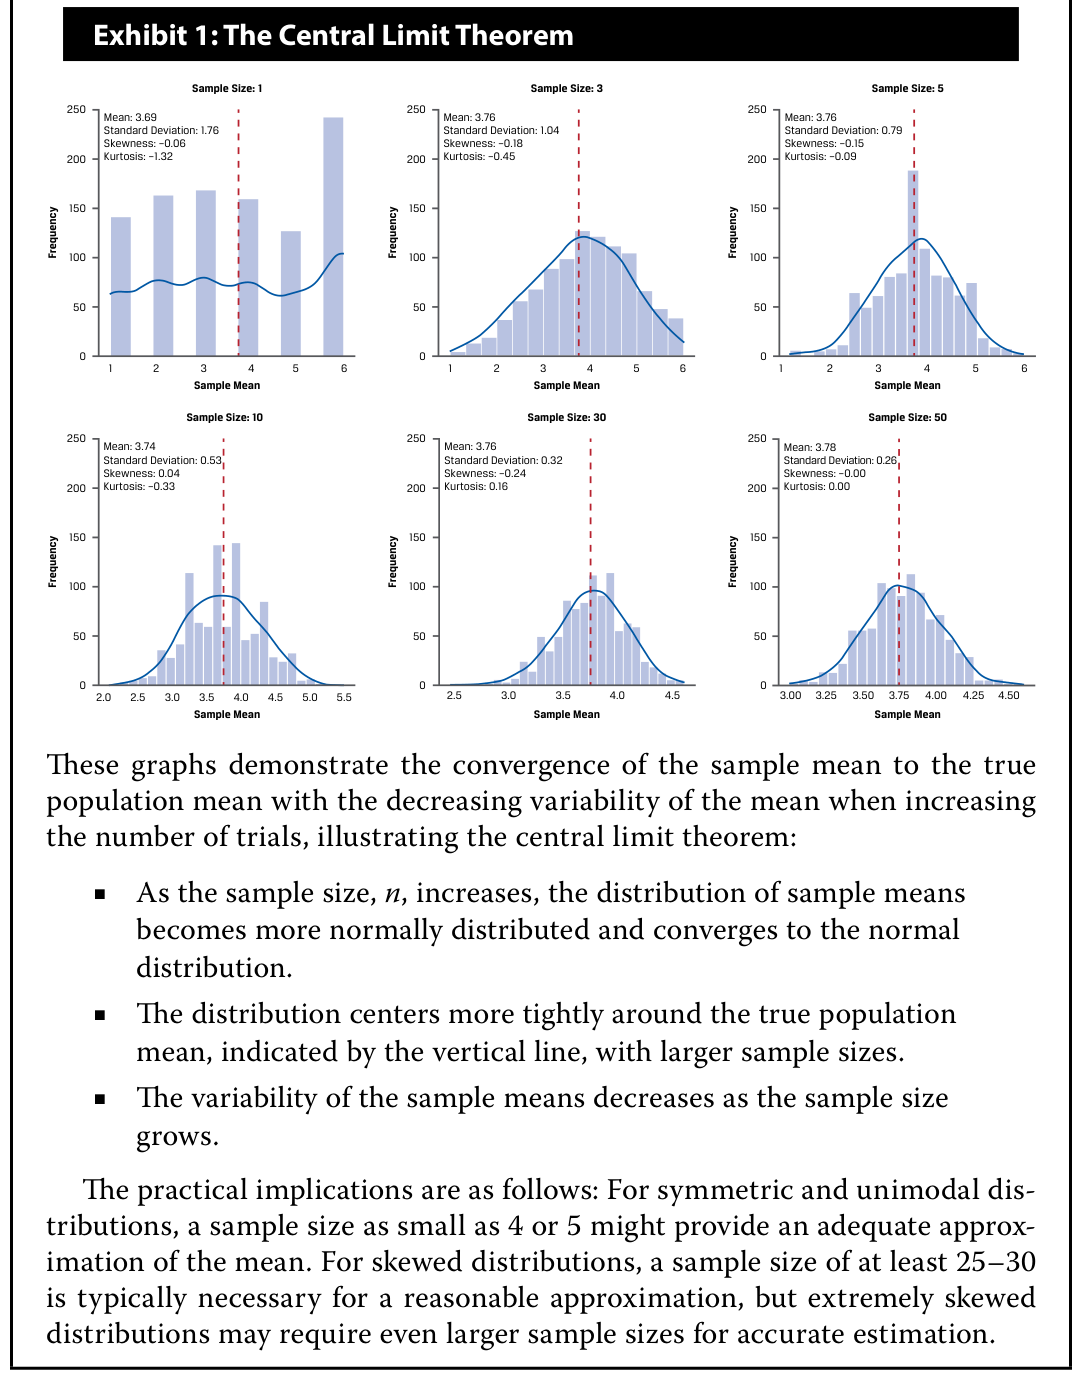
\includegraphics[width=0.85\linewidth]{002_figs/007_Module_7/exhibit_1.png}
	\caption{Histograms Showing the Convergence of the Sample Mean under CLT}
	\label{fig:mod7_exhibit_1}
\end{figure}
% Reference: CFA Curriculum 2027, Volume 1, Module 7, Page 324, Exhibit 1

An estimator $\hat{\theta}$ is:
\begin{itemize}
	\item \textbf{Unbiased} if $E[\hat{\theta}] = \theta$. The sample mean is an unbiased estimator of the population mean ($E[\bar{X}] = \mu$).
	\item \textbf{Efficient} if it has the smallest possible standard error among all unbiased estimators. A minimum-variance unbiased estimator (MVUE) is both unbiased and efficient. The best linear unbiased estimator (BLUE) is both unbiased and maximally efficient among all linear estimators.
	\item \textbf{Consistent} if it converges to the true parameter value as the sample size increases. The sample mean $\bar{X}$ is a consistent estimator.
	\item \textbf{Robust} if it provides accurate parameter estimates even when the data include outliers or violate distribution assumptions (e.g., using trimmed means).
\end{itemize}

\subsection{Confidence Intervals}
Confidence intervals are probabilistic ranges that are likely to contain the true parameter value with a specified level of confidence ($1 - \alpha$). For large sample sizes, the confidence interval for the population mean $\mu$ is:
\begin{equation}
	\bar{X} \pm Z_{\alpha/2} \times \frac{\sigma}{\sqrt{n}}
	\label{eq:confidence_interval_z_m7}
\end{equation}
% Reference: CFA Curriculum 2027, Volume 1, Module 7, Page 325, Equation (4)

Where $Z_{\alpha/2}$ is the critical Z-score from the normal distribution, and $\sigma/\sqrt{n}$ is the standard error. Exhibit~\ref{fig:mod7_exhibit_2} illustrates the normal distribution curve and confidence intervals.

\begin{figure}[!htbp]
	\centering
	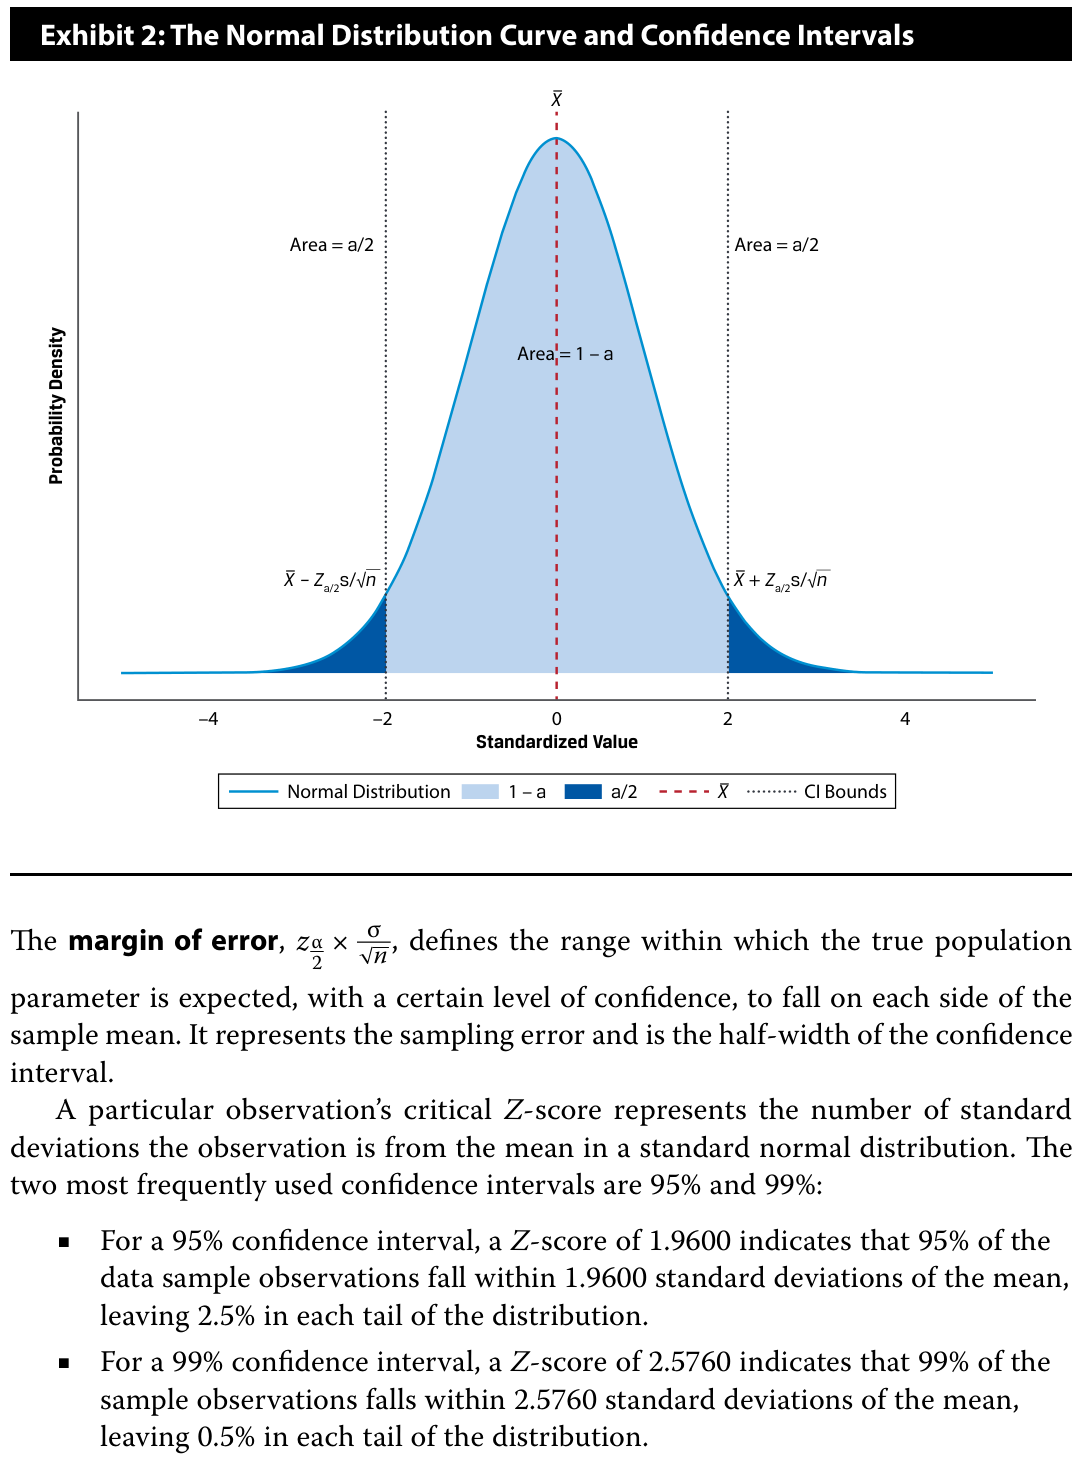
\includegraphics[width=0.75\linewidth]{002_figs/007_Module_7/exhibit_2.png}
	\caption{The Normal Distribution Curve and Confidence Intervals}
	\label{fig:mod7_exhibit_2}
\end{figure}
% Reference: CFA Curriculum 2027, Volume 1, Module 7, Page 326, Exhibit 2

The margin of error, $Z_{\alpha/2} \times \frac{\sigma}{\sqrt{n}}$, is the half-width of the confidence interval. The two most frequently used confidence intervals are:
\begin{itemize}
	\item \textbf{95\% Confidence Interval:} $Z_{0.025} = 1.9600$, leaving 2.5\% in each tail.
	\item \textbf{99\% Confidence Interval:} $Z_{0.005} = 2.5760$, leaving 0.5\% in each tail.
\end{itemize}

\begin{tcolorbox}[
	colback=gray!5!white,
	colframe=black!15!white,
	boxrule=0.5pt,
	arc=3pt,
	title=\textbf{Case Study: Estimating the Monthly Return on Gold},
	coltitle=black,
	colbacktitle=black!5!white,
	before skip=6pt,
	after skip=6pt,
	breakable
]
Based on 34 years of monthly returns on gold ($n = 408$), the average monthly return is $0.49\%$ and the sample standard deviation is $4.38\%$.
\begin{enumerate}
	\item \textbf{Standard Error:} $SE = \frac{s}{\sqrt{n}} = \frac{0.0438}{\sqrt{408}} \approx 0.0022$ (or $0.22\%$).
	\item \textbf{95\% Confidence Interval:} $0.49\% \pm 1.9600 \times 0.22\% = 0.49\% \pm 0.43\% \implies [0.06\%, 0.92\%]$.
	\item \textbf{99\% Confidence Interval:} $0.49\% \pm 2.5760 \times 0.22\% = 0.49\% \pm 0.57\% \implies [-0.08\%, 1.06\%]$.
\end{enumerate}
These intervals are shown in Exhibit~\ref{fig:mod7_exhibit_3}. Higher confidence levels result in wider confidence intervals.
\end{tcolorbox}

\begin{figure}[!htbp]
	\centering
	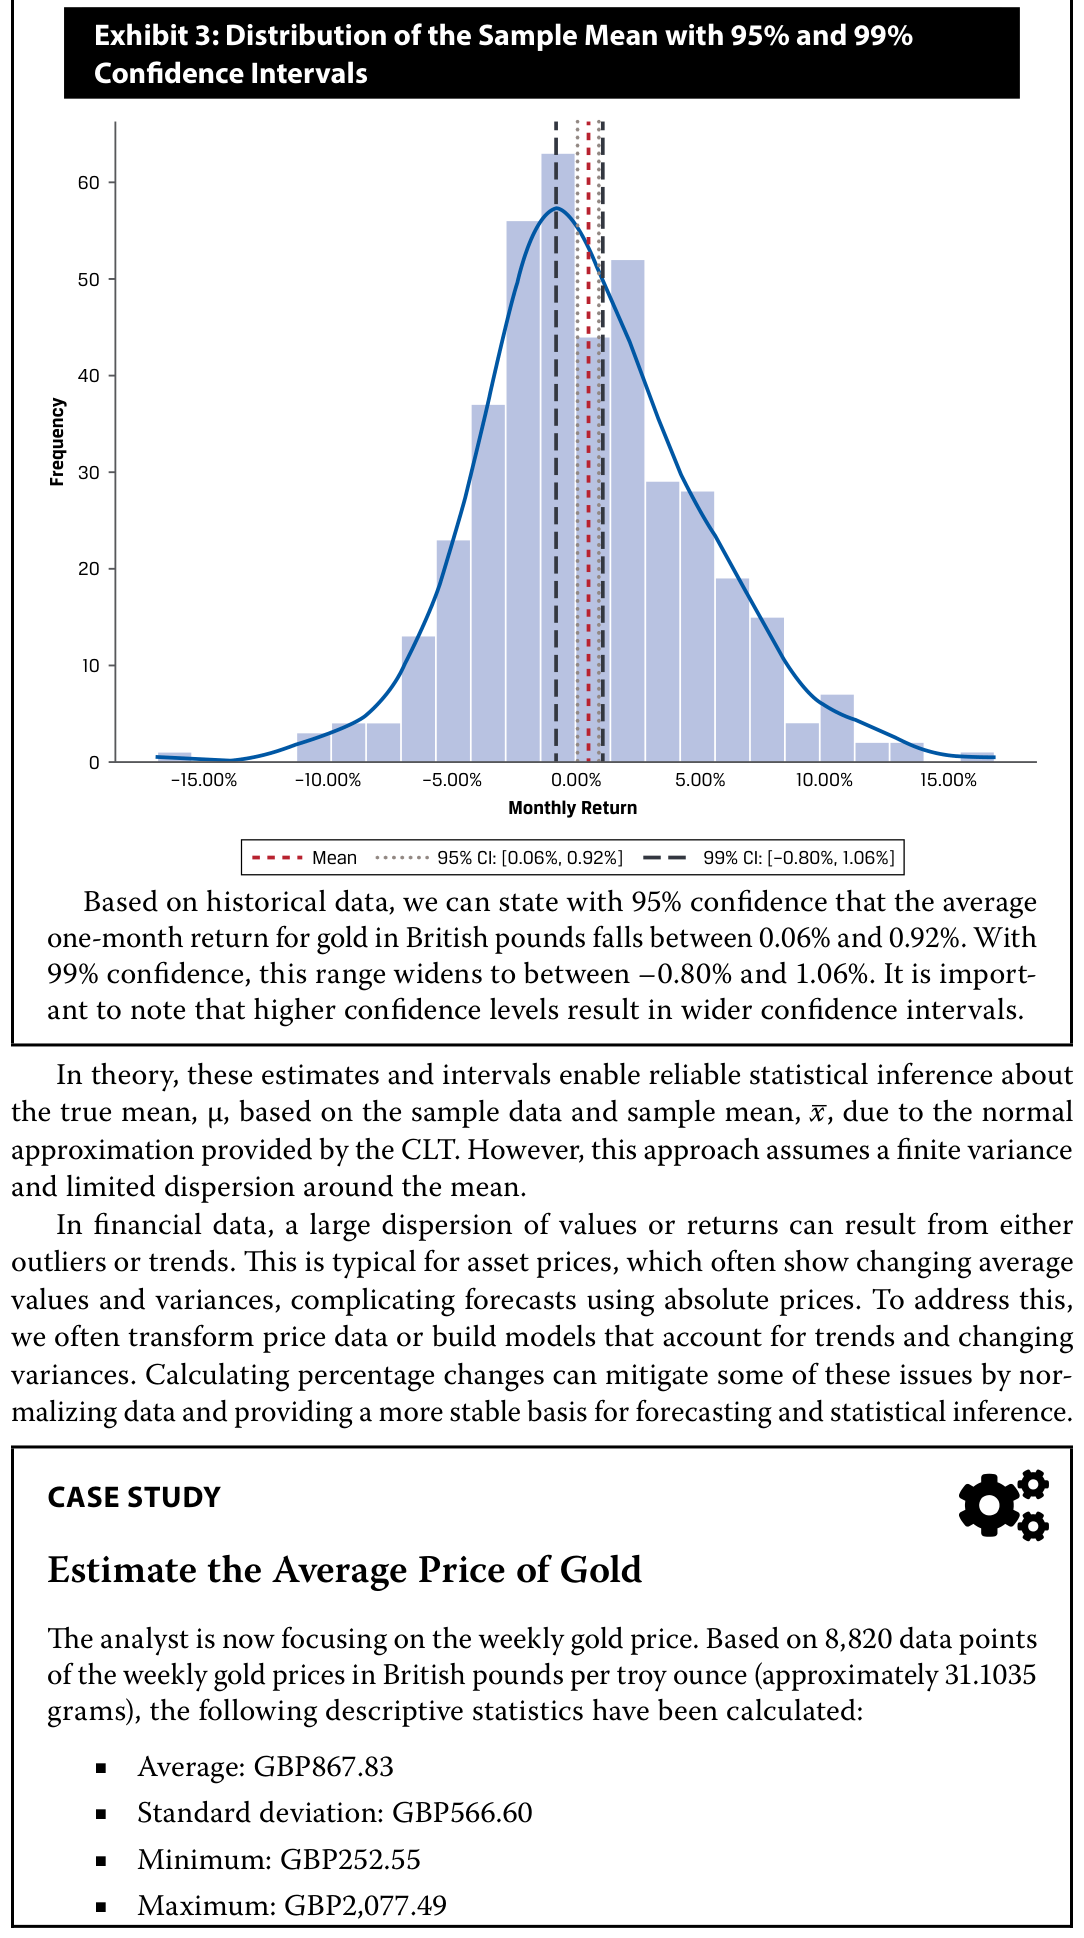
\includegraphics[width=0.75\linewidth]{002_figs/007_Module_7/exhibit_3.png}
	\caption{Distribution of the Sample Mean with 95\% and 99\% Confidence Intervals}
	\label{fig:mod7_exhibit_3}
\end{figure}
% Reference: CFA Curriculum 2027, Volume 1, Module 7, Page 328, Exhibit 3

\begin{tcolorbox}[
	colback=gray!5!white,
	colframe=black!15!white,
	boxrule=0.5pt,
	arc=3pt,
	title=\textbf{Case Study: Estimating the Average Price of Gold},
	coltitle=black,
	colbacktitle=black!5!white,
	before skip=6pt,
	after skip=6pt,
	breakable
]
Based on 8,820 weekly gold price data points, the average is GBP 867.83 and standard deviation is GBP 566.60 (Exhibit~\ref{fig:mod7_exhibit_4}). The distribution of prices is bimodal and highly skewed. This violates the normal distribution assumption of the CLT, making absolute price confidence intervals unreliable. Thus, transforming data into returns (percentage changes) is necessary to stabilize the variance.
\end{tcolorbox}

\begin{figure}[!htbp]
	\centering
	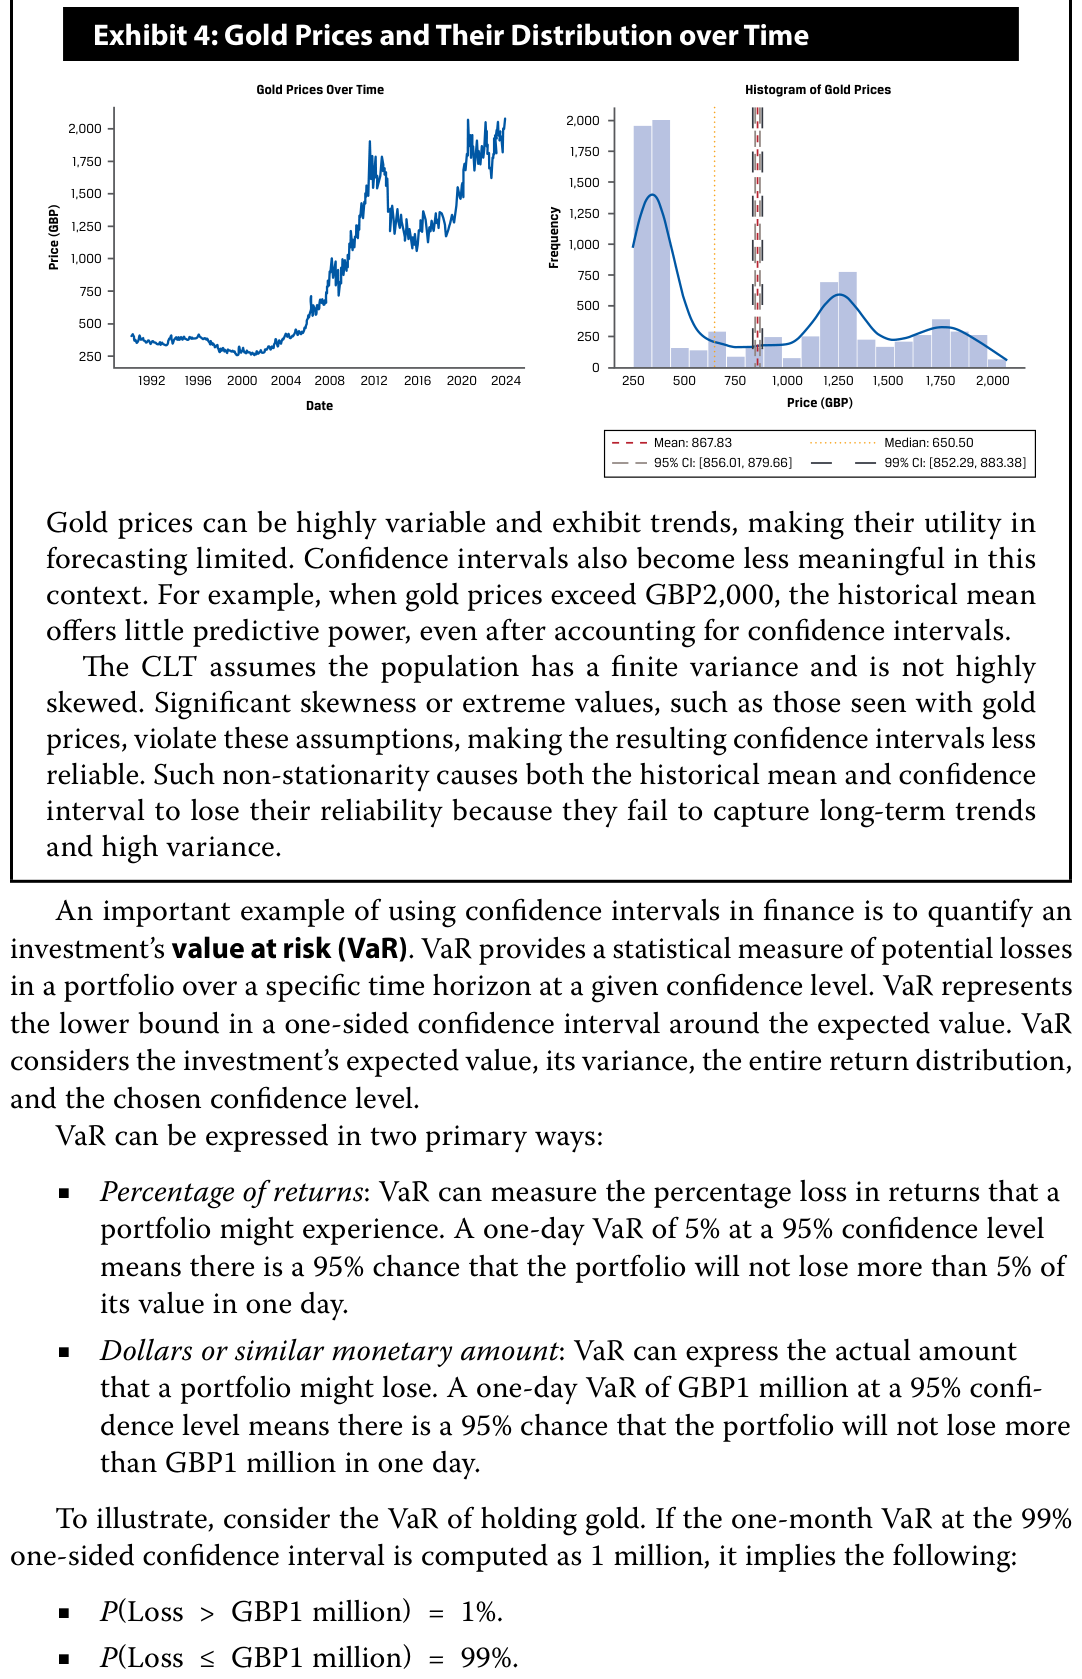
\includegraphics[width=0.85\linewidth]{002_figs/007_Module_7/exhibit_4.png}
	\caption{Gold Prices and Their Bimodal Distribution over Time}
	\label{fig:mod7_exhibit_4}
\end{figure}
% Reference: CFA Curriculum 2027, Volume 1, Module 7, Page 329, Exhibit 4

\begin{examtip}
\textbf{Value at Risk (VaR) as a One-Sided Confidence Interval}\\
VaR provides a statistical measure of potential losses in a portfolio over a specific time horizon at a given confidence level. It represents the lower bound of a one-sided confidence interval.
\begin{itemize}
	\item $P(\text{Loss} > \text{VaR}) = \alpha$
	\item $P(\text{Loss} \le \text{VaR}) = 1 - \alpha$
\end{itemize}
Assuming normally distributed asset returns and a mean return of zero, the parametric VaR is:
\begin{equation}
	\text{VaR} = Z_{\alpha} \times \sigma \times P
	\label{eq:var_formula_m7}
\end{equation}
% Reference: CFA Curriculum 2027, Volume 1, Module 7, Page 330, Equation (5)
Where $Z_{\alpha}$ corresponds to the one-sided percentile (e.g., $1.65$ for 95\%, $2.33$ for 99\%), $\sigma$ is standard deviation, and $P$ is the current position value (Exhibit~\ref{fig:mod7_exhibit_5}).
\end{examtip}

\begin{figure}[!htbp]
	\centering
	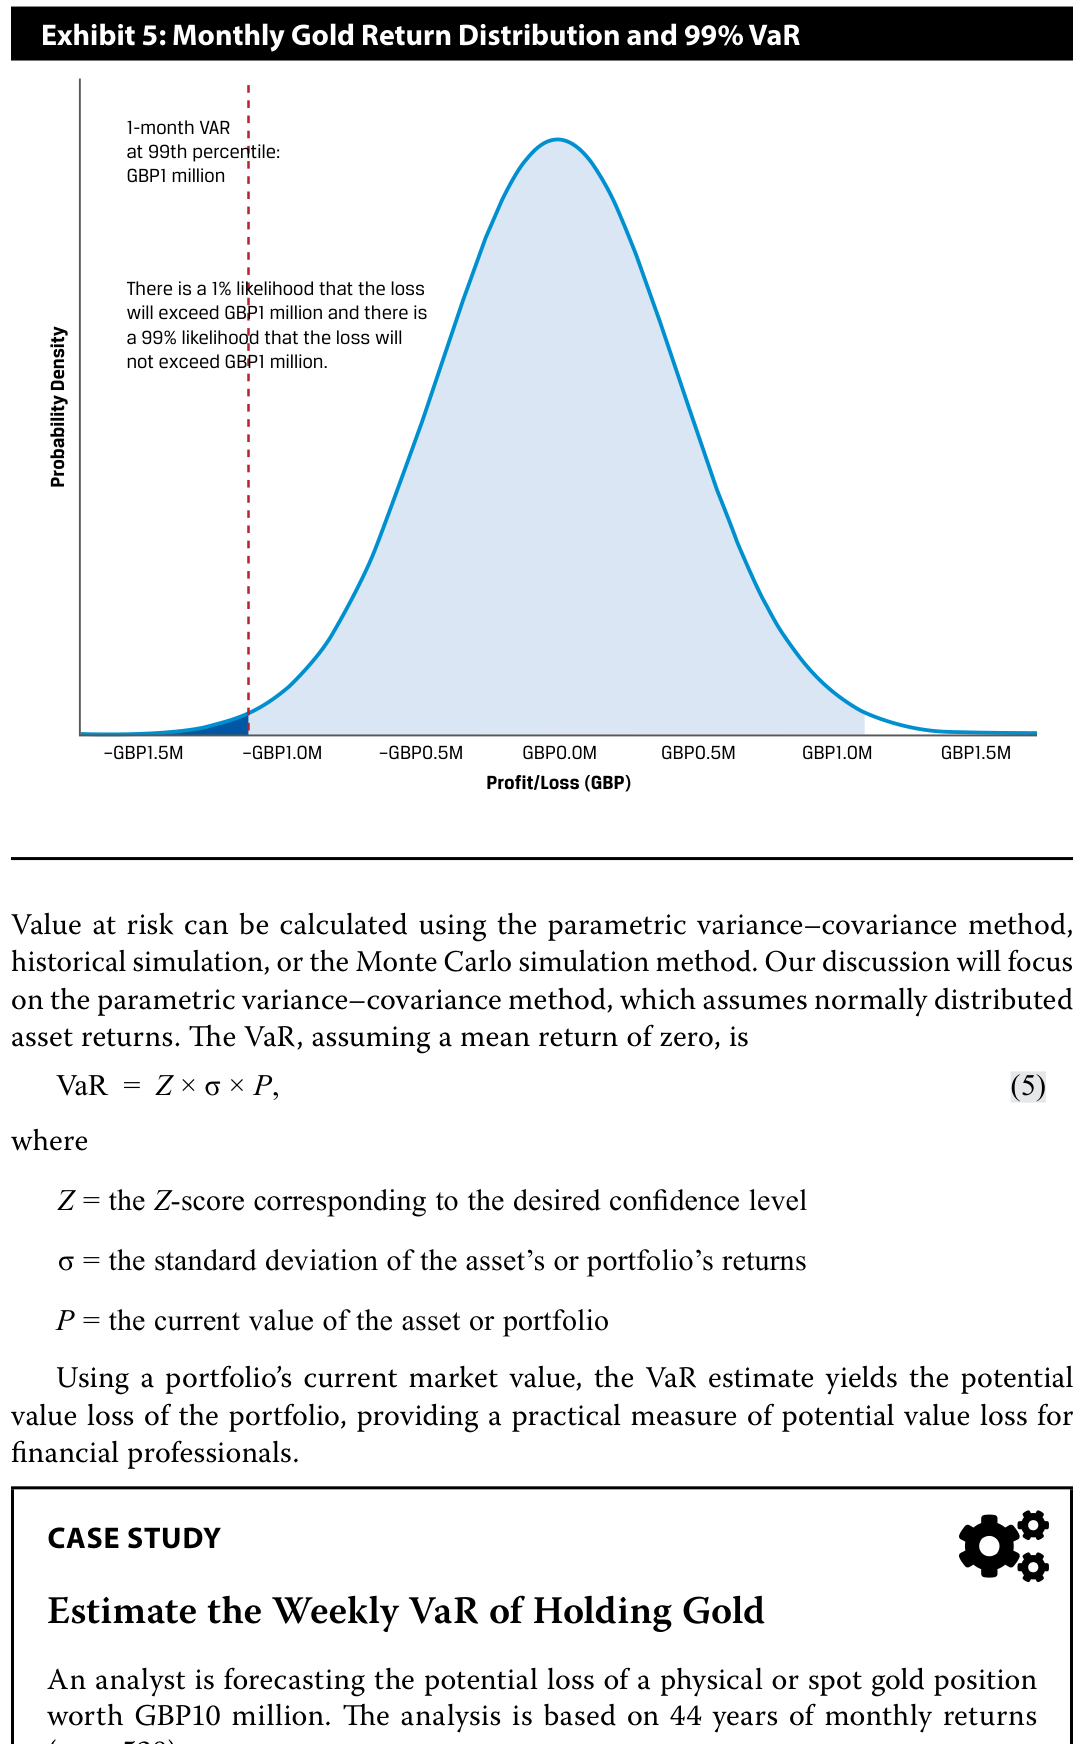
\includegraphics[width=0.75\linewidth]{002_figs/007_Module_7/exhibit_5.png}
	\caption{Monthly Gold Return Distribution and 99\% VaR}
	\label{fig:mod7_exhibit_5}
\end{figure}
% Reference: CFA Curriculum 2027, Volume 1, Module 7, Page 330, Exhibit 5

\begin{tcolorbox}[
	colback=gray!5!white,
	colframe=black!15!white,
	boxrule=0.5pt,
	arc=3pt,
	title=\textbf{Case Study: Estimating the Weekly VaR of Gold},
	coltitle=black,
	colbacktitle=black!5!white,
	before skip=6pt,
	after skip=6pt,
	breakable
]
An analyst forecasts potential loss of a spot gold position worth GBP 10 million. Monthly standard deviation is $5.02\%$. Assuming a mean return of 0\% and normal distribution, the 99\% one-month VaR is:
\[ \text{VaR} = 2.33 \times 5.02\% \times \text{GBP } 10,000,000 = \text{GBP } 1,169,660 \]
There is a 1\% probability that the position will lose more than GBP 1,169,660 over the next month.
\end{tcolorbox}

\subsection{Sampling Methodologies}
To extract information about a population, two sampling approaches can be used:
\begin{enumerate}
	\item \textbf{Probability Sampling:} Every member of the population has a known, non-zero chance of selection.
	      \begin{itemize}
		      \item \textbf{Simple Random Sampling:} Each element has an equal selection chance.
		      \item \textbf{Systematic Sampling:} Selects every $k$-th member of a population.
		      \item \textbf{Stratified Random Sampling:} Divides the population into strata based on criteria, then draws random samples proportionally from each stratum. This increases precision.
		      \item \textbf{Cluster Sampling:} Divides the population into small clusters, randomly selects clusters, and samples all members in selected clusters.
	      \end{itemize}
	\item \textbf{Non-Probability Sampling:} Relies on judgment or convenience; does not guarantee representativeness, so the CLT does not reliably apply.
	      \begin{itemize}
		      \item \textbf{Convenience Sampling:} Selecting accessible elements.
		      \item \textbf{Judgmental Sampling:} Selecting elements based on expertise.
	      \end{itemize}
\end{enumerate}

\begin{tcolorbox}[
	colback=gray!5!white,
	colframe=black!15!white,
	boxrule=0.5pt,
	arc=3pt,
	title=\textbf{Case Study: Sampling of Daily Returns},
	coltitle=black,
	colbacktitle=black!5!white,
	before skip=6pt,
	after skip=6pt,
	breakable
]
Based on 1,258 daily return observations of a global small-cap stock index, the true population mean is $0.035\%$. As shown in Exhibit~\ref{fig:mod7_exhibit_6}, mean absolute errors decrease rapidly as sample size $n$ increases. Stratified sampling (stratified by year) generally yields smaller errors than simple random sampling, although the advantage decreases as sample size grows.
\end{tcolorbox}

\begin{figure}[!htbp]
	\centering
	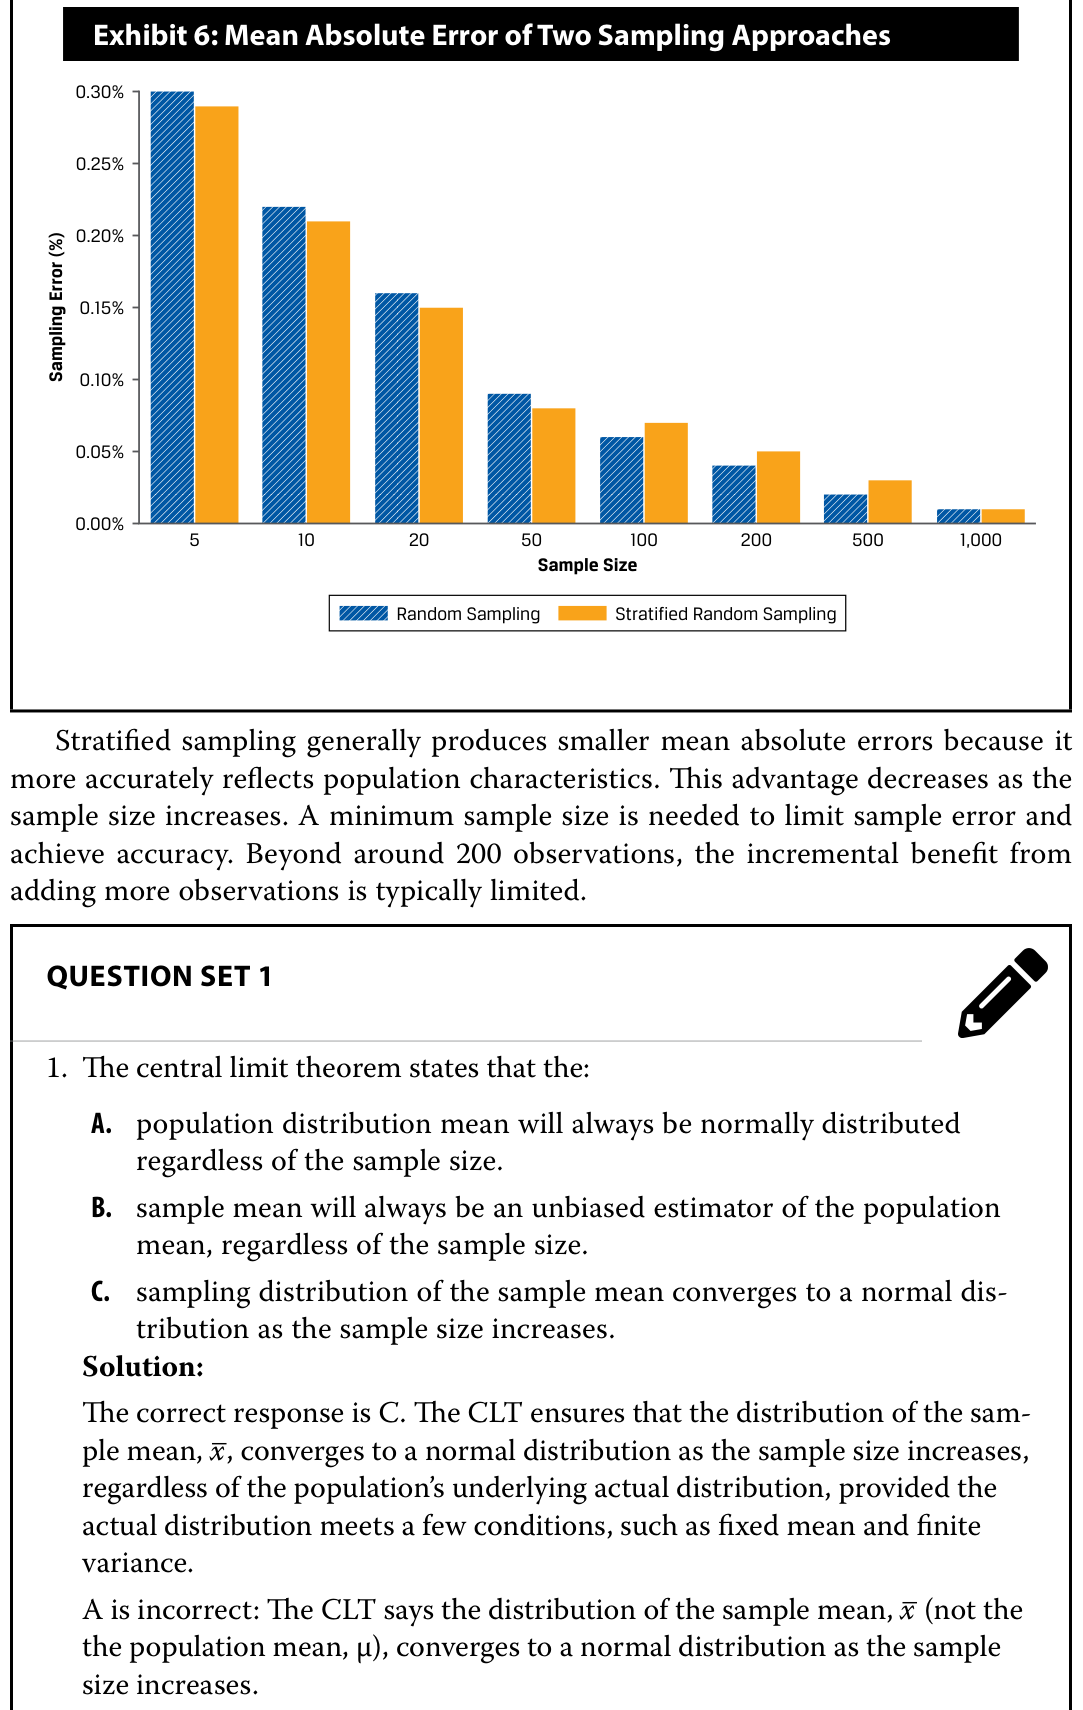
\includegraphics[width=0.75\linewidth]{002_figs/007_Module_7/exhibit_6.png}
	\caption{Mean Absolute Error of Random vs Stratified Sampling}
	\label{fig:mod7_exhibit_6}
\end{figure}
% Reference: CFA Curriculum 2027, Volume 1, Module 7, Page 334, Exhibit 6

\section{HYPOTHESIS TESTING AND PARAMETRIC TESTING}
\begin{center}
\begin{tabular}{p{0.06\linewidth} | p{0.88\linewidth}}
	b & explain hypothesis testing and its components, including statistical significance, Type I and Type II errors, and the power of a test; construct appropriate hypothesis tests; and interpret the results \\
\end{tabular}
\end{center}

\textcolor{blue}{\textit{Quy trình kiểm định giả thuyết gồm 4 bước (Exhibit~\ref{fig:mod7_exhibit_7}). Chúng ta đặc biệt lưu ý lỗi Loại I ($\alpha$ - bác bỏ $H_0$ đúng), lỗi Loại II ($\beta$ - không bác bỏ $H_0$ sai) và lực lượng kiểm định ($1 - \beta$). Nhớ phân phối tương ứng: kiểm định trung bình ($t$), một phương sai ($\chi^2$), hai phương sai ($F$).}}

\subsection{The Hypothesis Testing Process}
Hypothesis testing involves four steps, as outlined in Exhibit~\ref{fig:mod7_exhibit_7}:
\begin{enumerate}
	\item State the null hypothesis ($H_0$) and alternative hypothesis ($H_A$).
	\item Identify the test statistic and its probability distribution.
	\item Specify the level of significance ($\alpha$).
	\item Establish the decision rule, calculate the statistic, and make the decision.
\end{enumerate}

\begin{figure}[!htbp]
	\centering
	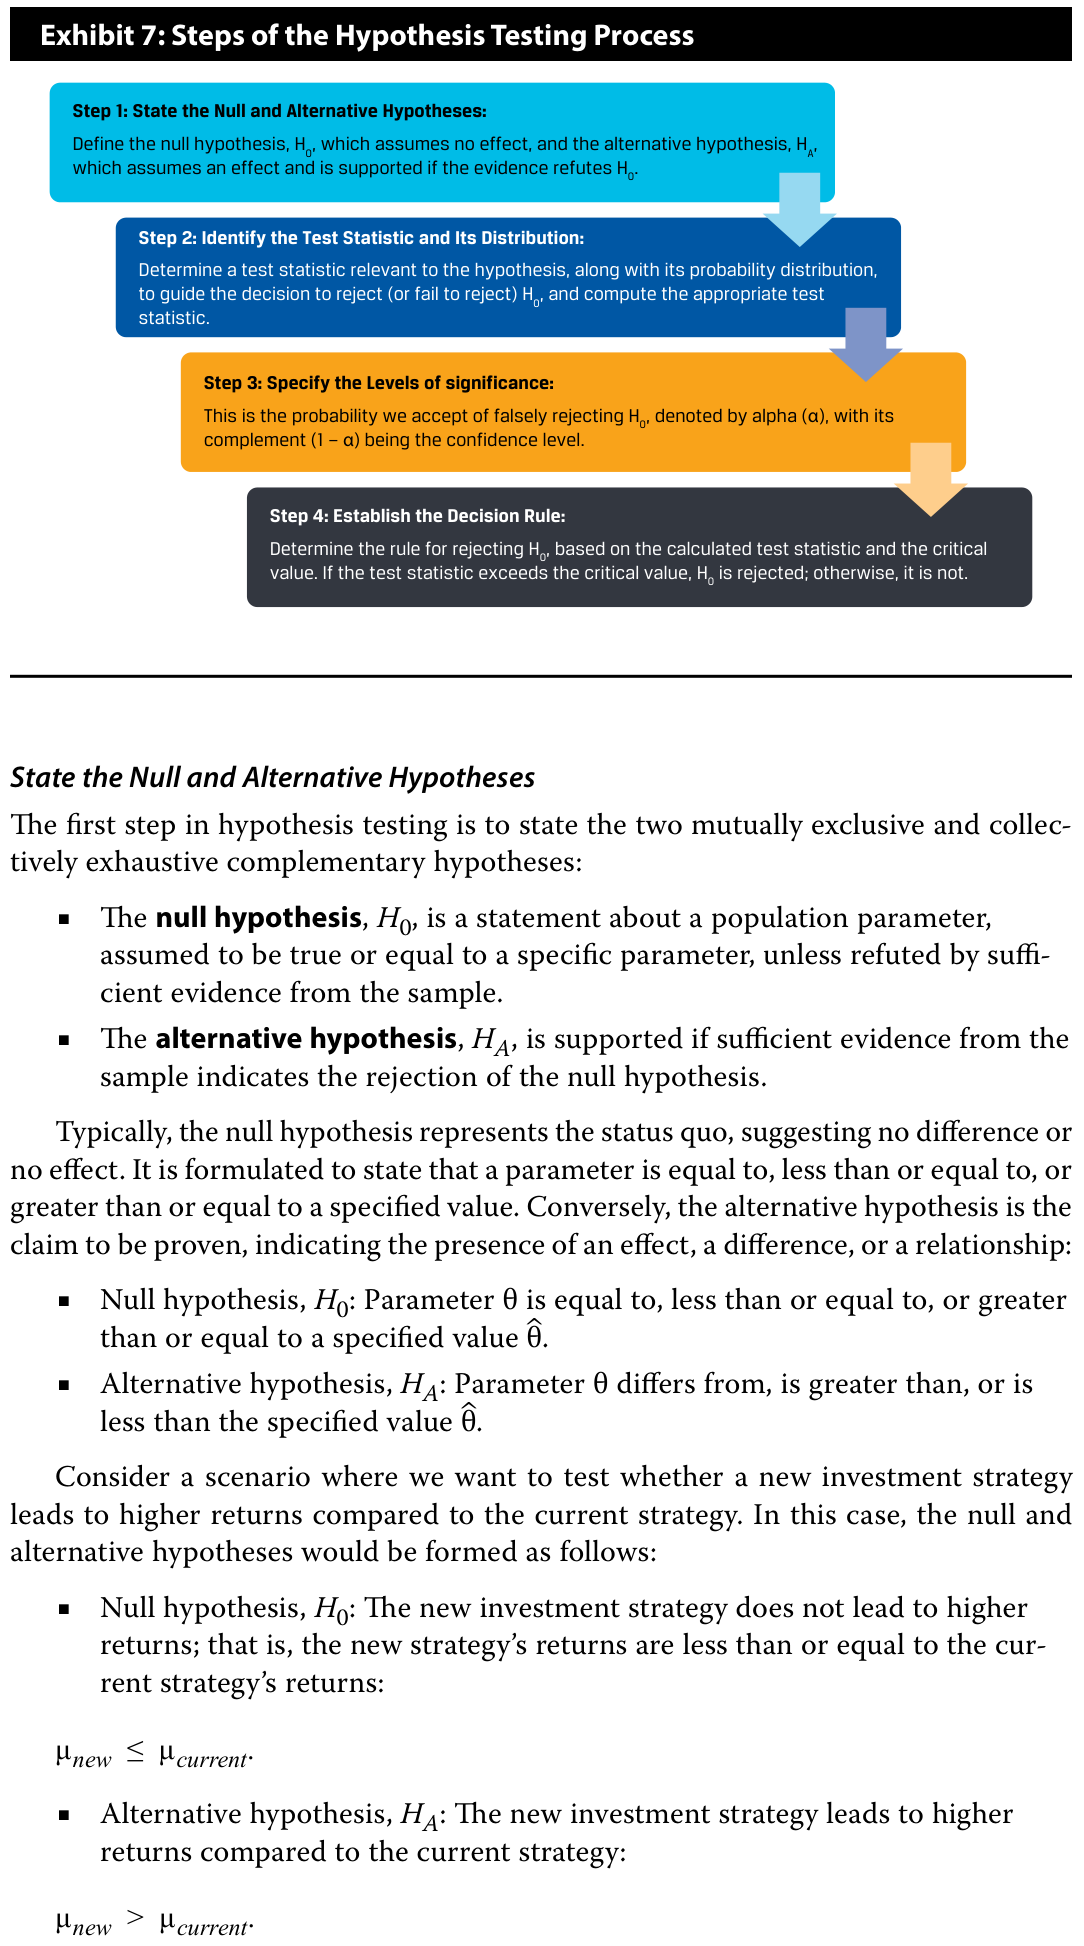
\includegraphics[width=0.7\linewidth]{002_figs/007_Module_7/exhibit_7.png}
	\caption{Steps of the Hypothesis Testing Process}
	\label{fig:mod7_exhibit_7}
\end{figure}
% Reference: CFA Curriculum 2027, Volume 1, Module 7, Page 337, Exhibit 7

\begin{figure}[!htbp]
	\centering
	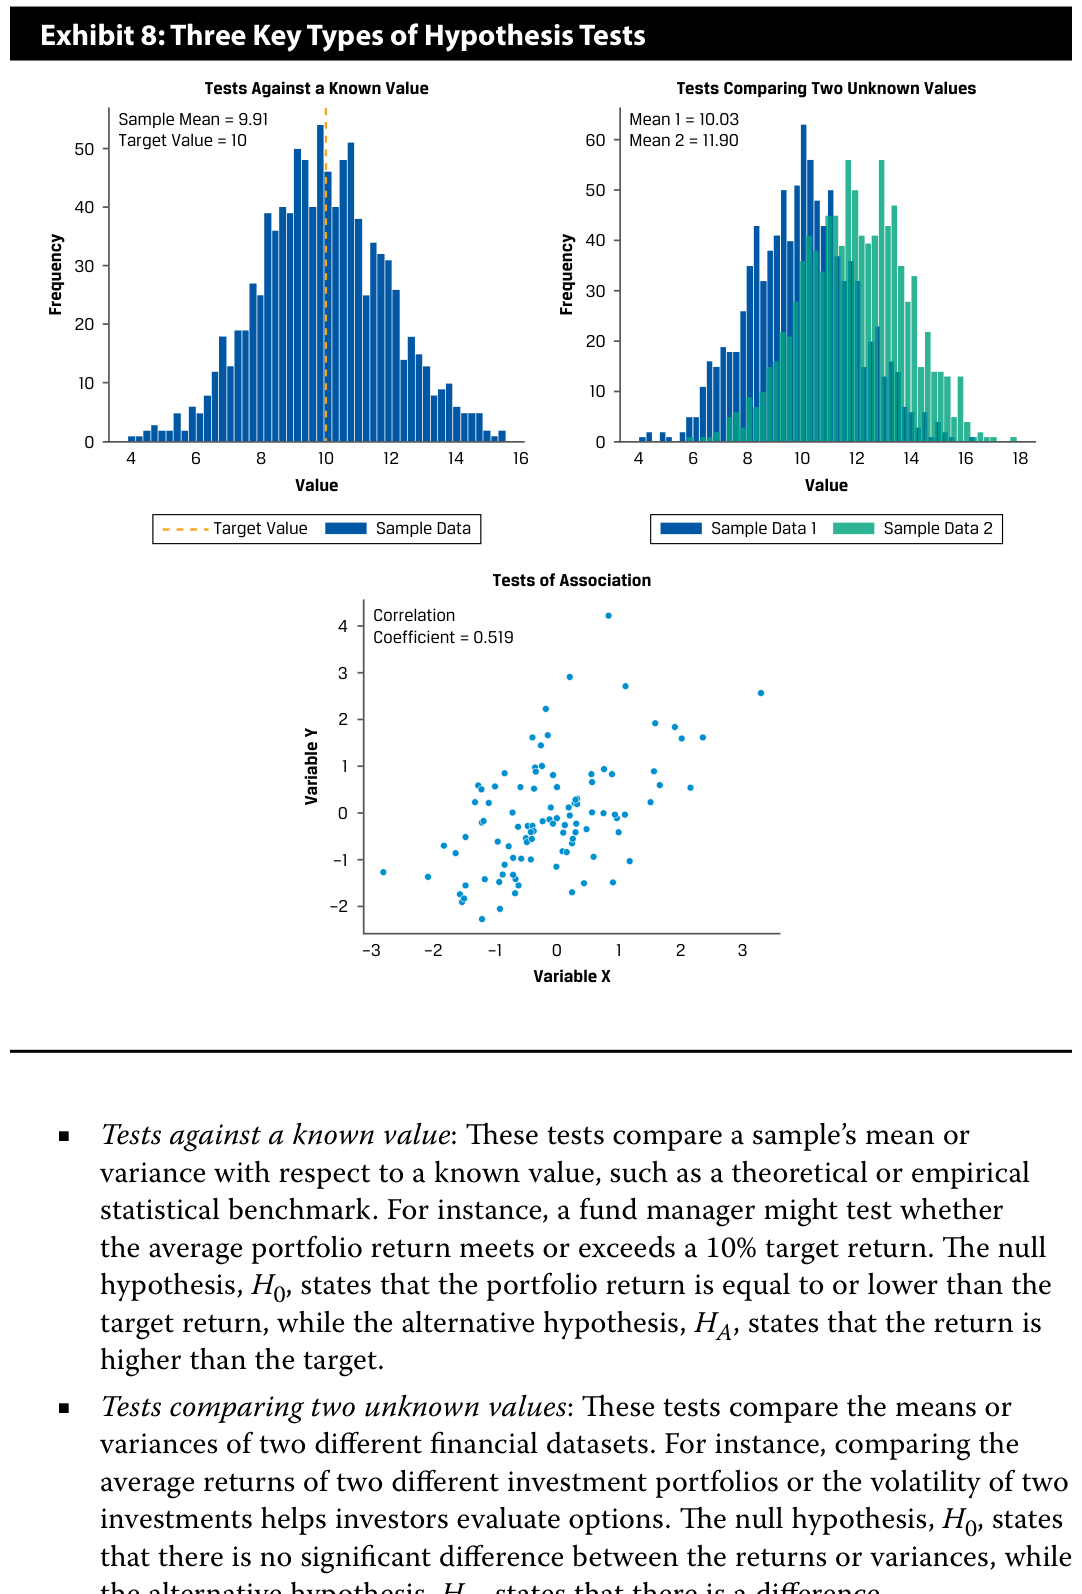
\includegraphics[width=0.75\linewidth]{002_figs/007_Module_7/exhibit_8.png}
	\caption{Three Key Types of Hypothesis Tests}
	\label{fig:mod7_exhibit_8}
\end{figure}
% Reference: CFA Curriculum 2027, Volume 1, Module 7, Page 338, Exhibit 8

Hypothesis tests can be formulated in three ways (Exhibit~\ref{fig:mod7_exhibit_8} \& Exhibit~\ref{tab:hypotheses_types_m7}):
\begin{itemize}
	\item \textbf{Right-tail test:} Tests whether a parameter $\theta$ is significantly greater than $\theta_0$ ($H_0: \theta \le \theta_0$ vs $H_A: \theta > \theta_0$).
	\item \textbf{Left-tail test:} Tests whether a parameter $\theta$ is significantly less than $\theta_0$ ($H_0: \theta \ge \theta_0$ vs $H_A: \theta < \theta_0$).
	\item \textbf{Two-tailed test:} Tests whether a parameter $\theta$ is significantly different from $\theta_0$ ($H_0: \theta = \theta_0$ vs $H_A: \theta \ne \theta_0$).
\end{itemize}

\begin{table}[!htbp]
\centering
\caption{General Formulation of Hypotheses}
\label{tab:hypotheses_types_m7}
\begin{tabular}{p{0.20\linewidth} p{0.38\linewidth} p{0.18\linewidth} p{0.14\linewidth}}
\toprule
\textbf{Test Type} & \textbf{Null Hypothesis ($H_0$)} & \textbf{Alternative ($H_A$)} & \textbf{Rejection Region} \\
\midrule
\textbf{Right-tail test} & $\theta \le \theta_0$ & $\theta > \theta_0$ & Right tail \\
\textbf{Left-tail test} & $\theta \ge \theta_0$ & $\theta < \theta_0$ & Left tail \\
\textbf{Two-tailed test} & $\theta = \theta_0$ & $\theta \ne \theta_0$ & Both tails \\
\bottomrule
\end{tabular}
\end{table}
% Reference: CFA Curriculum 2027, Volume 1, Module 7, Page 339, Exhibit 9

Exhibit~\ref{fig:mod7_exhibit_10} depicts the rejection areas for the three types of hypothesis tests.

\begin{figure}[!htbp]
	\centering
	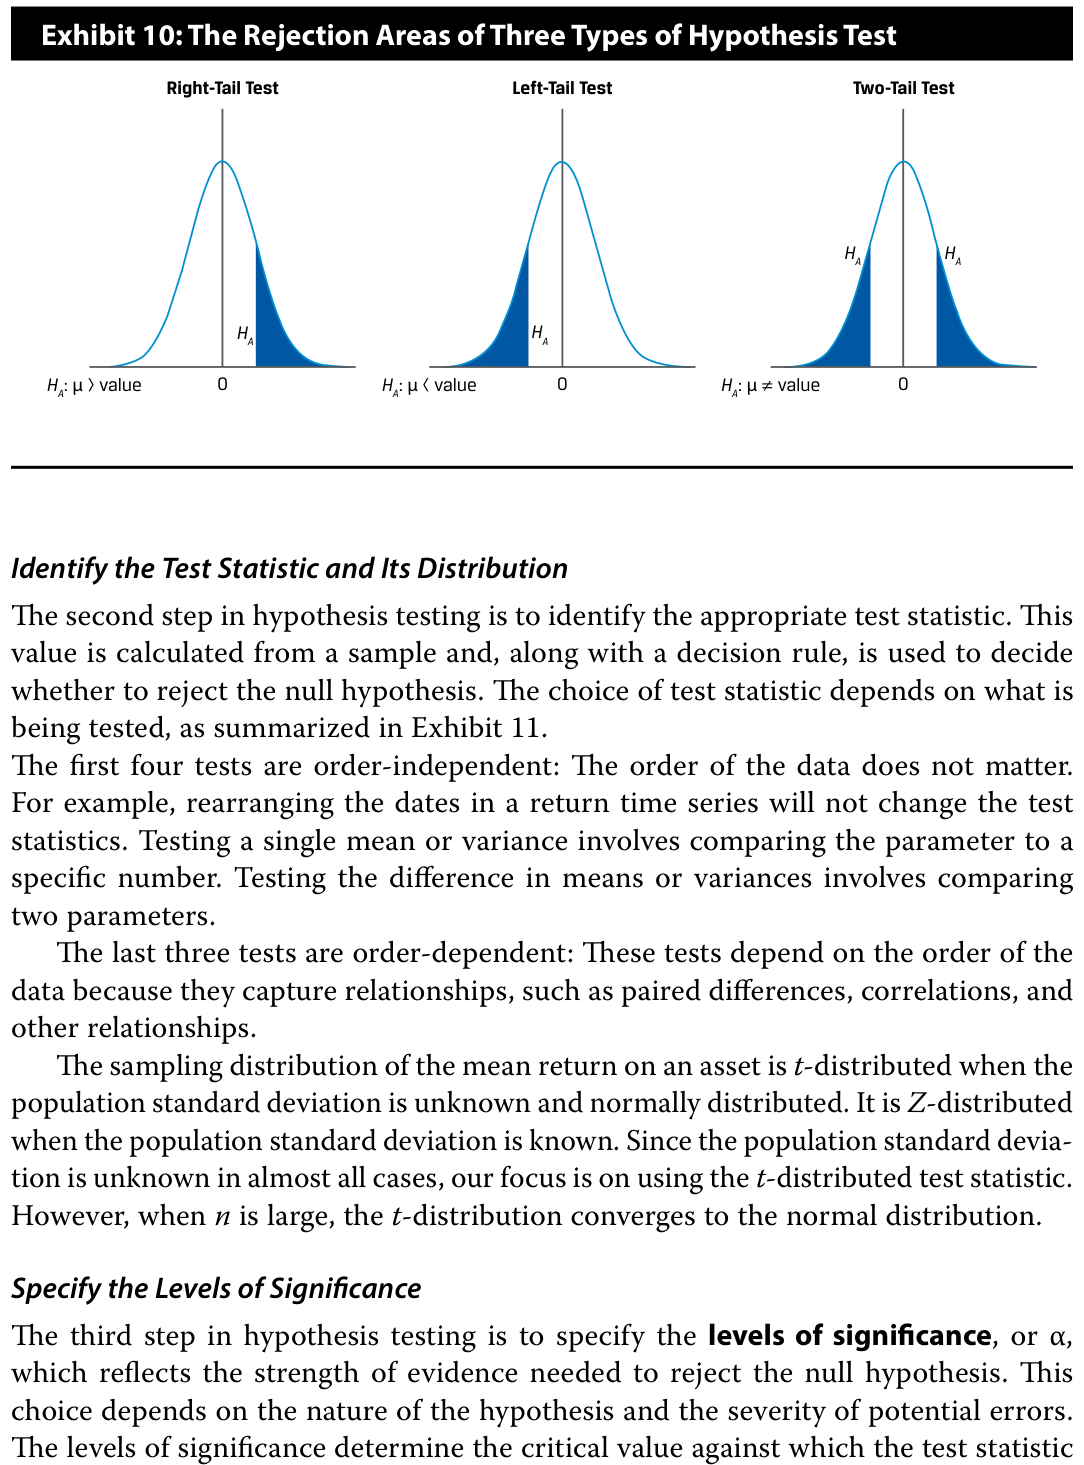
\includegraphics[width=0.85\linewidth]{002_figs/007_Module_7/exhibit_10.png}
	\caption{Rejection Regions for One-Tailed and Two-Tailed Tests}
	\label{fig:mod7_exhibit_10}
\end{figure}
% Reference: CFA Curriculum 2027, Volume 1, Module 7, Page 340, Exhibit 10

\subsection{Type I and Type II Errors}
The decision-making process in hypothesis testing involves two types of errors:
\begin{itemize}
	\item \textbf{Type I Error (False Positive):} Rejecting a true null hypothesis. The probability of a Type I error is the level of significance, $\alpha$.
	\item \textbf{Type II Error (False Negative):} Failing to reject a false null hypothesis. The probability of a Type II error is denoted by $\beta$.
\end{itemize}

\begin{table}[!htbp]
\centering
\caption{Decisions in Hypothesis Testing}
\label{tab:decision_matrix_m7}
\begin{tabular}{p{0.28\linewidth} | p{0.32\linewidth} | p{0.32\linewidth}}
\toprule
\textbf{Decision} & \textbf{Null Hypothesis ($H_0$) is True} & \textbf{Null Hypothesis ($H_0$) is False} \\
\midrule
\textbf{Fail to reject $H_0$} & Correct Decision ($1 - \alpha$) & Type II Error ($\beta$, False Negative) \\
\midrule
\textbf{Reject $H_0$} & Type I Error ($\alpha$, False Positive) & Correct Decision ($1 - \beta$, Power of the Test) \\
\bottomrule
\end{tabular}
\end{table}
% Reference: CFA Curriculum 2027, Volume 1, Module 7, Page 342, Exhibit 12

The relation between $\alpha$ and $\beta$ is shown in Exhibit~\ref{fig:mod7_exhibit_13}. Reducing $\alpha$ increases $\beta$ for a fixed sample size. To decrease both errors simultaneously, we must increase the sample size $n$.

\begin{figure}[!htbp]
	\centering
	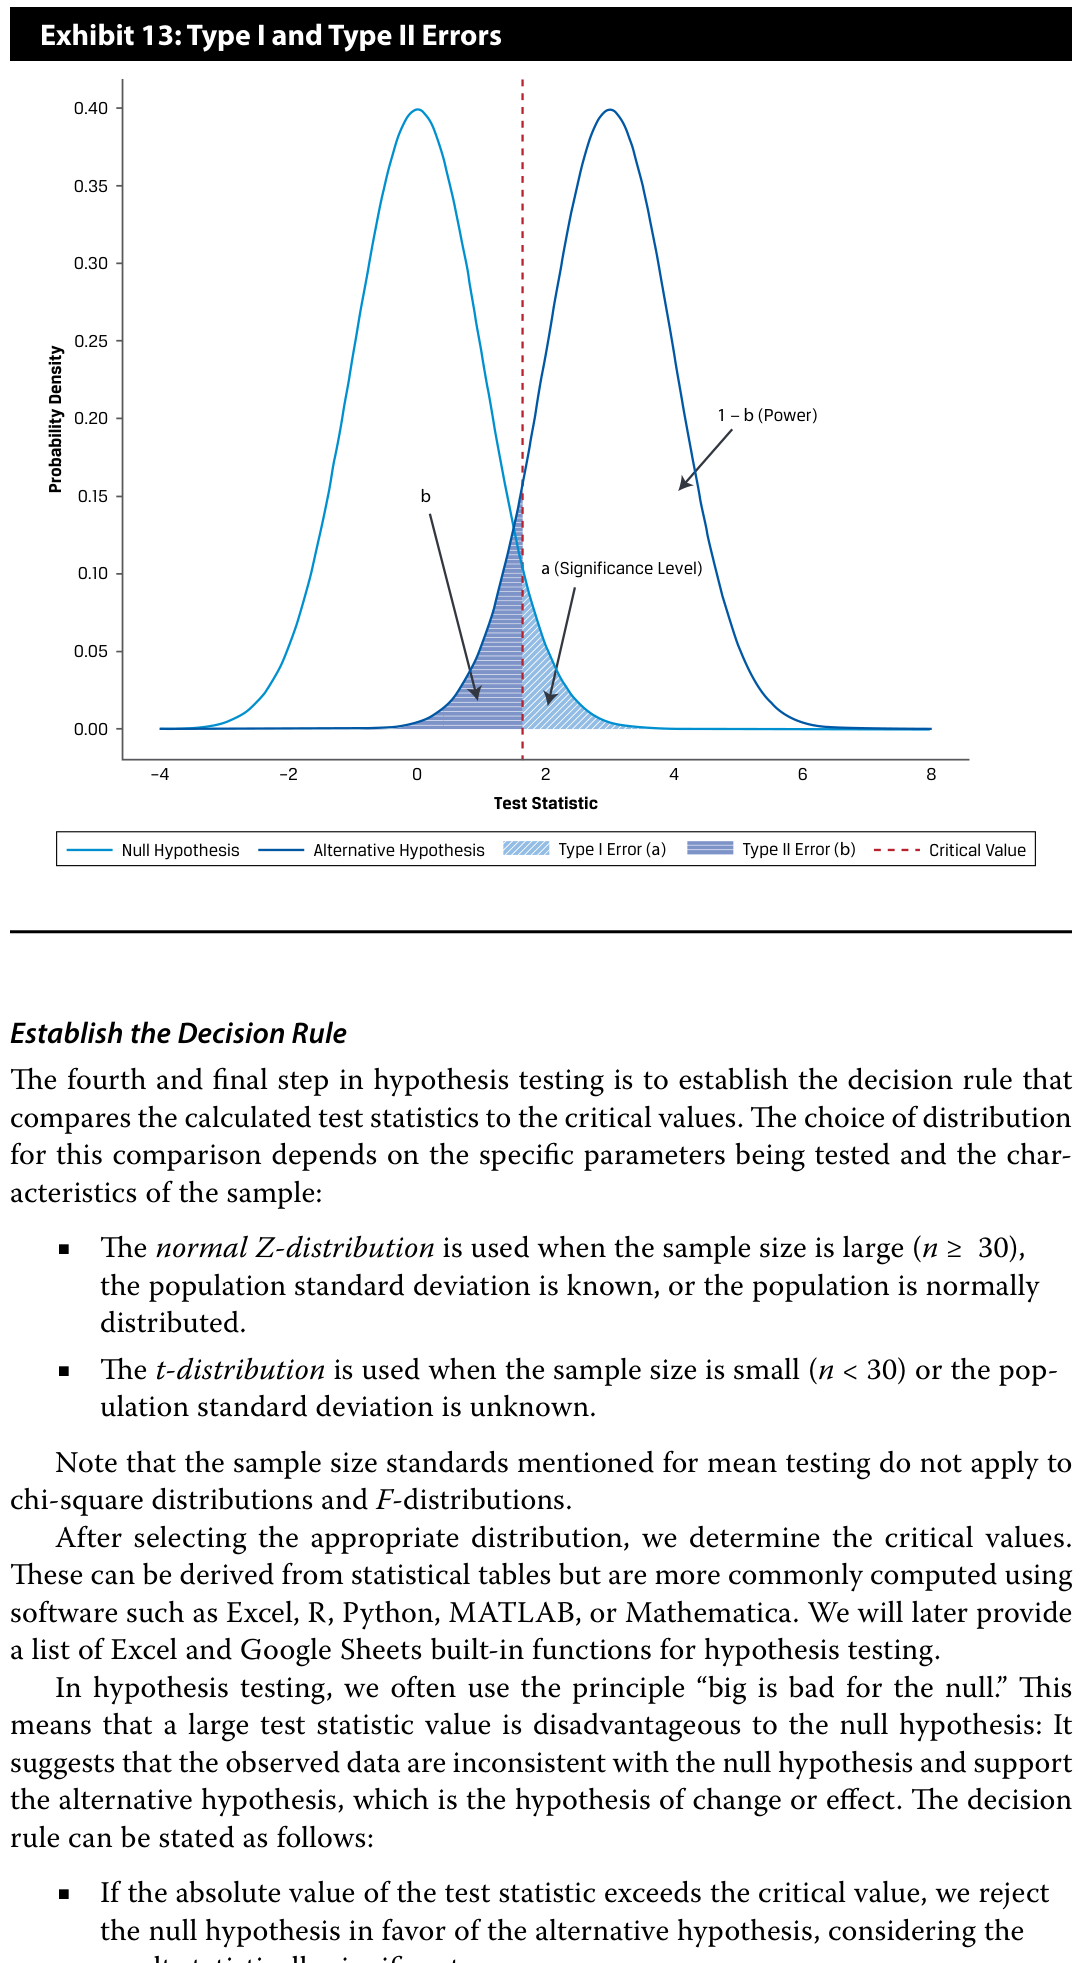
\includegraphics[width=0.75\linewidth]{002_figs/007_Module_7/exhibit_13.png}
	\caption{The Trade-Off Between Type I and Type II Errors}
	\label{fig:mod7_exhibit_13}
\end{figure}
% Reference: CFA Curriculum 2027, Volume 1, Module 7, Page 343, Exhibit 13

\subsection{Parametric Tests for a Single Variable}
We utilize annual return data from 1979 to 2023 ($n = 44$) for the MSCI World Value and Growth Indexes to illustrate parametric tests (Exhibit~\ref{fig:mod7_exhibit_14} \& Table~\ref{tab:msci_stats_m7}).

\begin{figure}[!htbp]
	\centering
	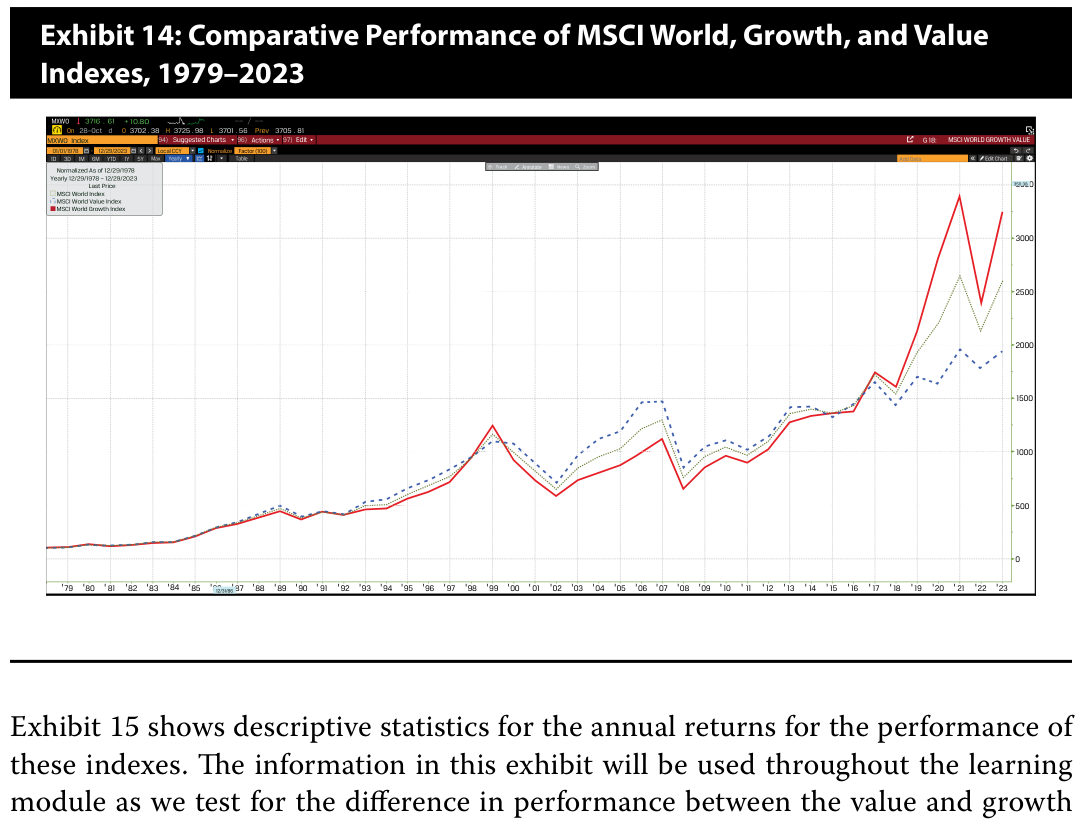
\includegraphics[width=0.85\linewidth]{002_figs/007_Module_7/exhibit_14.png}
	\caption{Performance of MSCI World, Growth, and Value Indexes, 1979--2023}
	\label{fig:mod7_exhibit_14}
\end{figure}
% Reference: CFA Curriculum 2027, Volume 1, Module 7, Page 345, Exhibit 14

\begin{table}[!htbp]
\centering
\caption{Descriptive Statistics for MSCI World, Value, and Growth Indexes}
\label{tab:msci_stats_m7}
\begin{tabular}{p{0.40\linewidth} p{0.16\linewidth} p{0.14\linewidth} p{0.15\linewidth}}
\toprule
\textbf{Metric} & \textbf{MSCI World} & \textbf{Growth Index} & \textbf{Value Index} \\
\midrule
Average annual return ($\bar{X}$) & 7.91\% & 8.81\% & 7.17\% \\
Sample variance ($s^2$) & 0.0381 & 0.0456 & 0.0362 \\
Sample standard deviation ($s$) & 0.1952 & 0.2134 & 0.1902 \\
Number of observations ($n$) & 44 & 44 & 44 \\
\bottomrule
\end{tabular}
\end{table}
% Reference: CFA Curriculum 2027, Volume 1, Module 7, Page 346, Exhibit 15

\subsubsection{Test of a Single Mean}
When the population standard deviation is unknown, the $t$-test statistic with $n - 1$ degrees of freedom is:
\begin{equation}
	t = \frac{\bar{X} - \mu_0}{s / \sqrt{n}}
	\label{eq:single_mean_t_test_m7}
\end{equation}
% Reference: CFA Curriculum 2027, Volume 1, Module 7, Page 346, Equation (6)

\begin{tcolorbox}[
	colback=gray!5!white,
	colframe=black!15!white,
	boxrule=0.5pt,
	arc=3pt,
	title=\textbf{Case Study: Testing MSCI World Value Index Mean Return},
	coltitle=black,
	colbacktitle=black!5!white,
	before skip=6pt,
	after skip=6pt,
	breakable
]
We test whether the average return of global value stocks is greater than zero ($H_0: \mu \le 0$ vs $H_A: \mu > 0$).
\begin{enumerate}
	\item \textbf{Calculate Test Statistic:} $t = \frac{0.0717 - 0}{0.1902 / \sqrt{44}} \approx 2.5001$.
	\item \textbf{Decision Rule ($df = 43$):} One-tailed critical values are $t_{0.05} = 1.6811$ and $t_{0.01} = 2.4163$ (Exhibit~\ref{fig:mod7_exhibit_16}).
	\item \textbf{Conclusion:} Since $2.5001 > 2.4163$, we reject $H_0$ at both the 5\% and 1\% levels. The average return is significantly greater than zero.
\end{enumerate}
\end{tcolorbox}

\begin{figure}[!htbp]
	\centering
	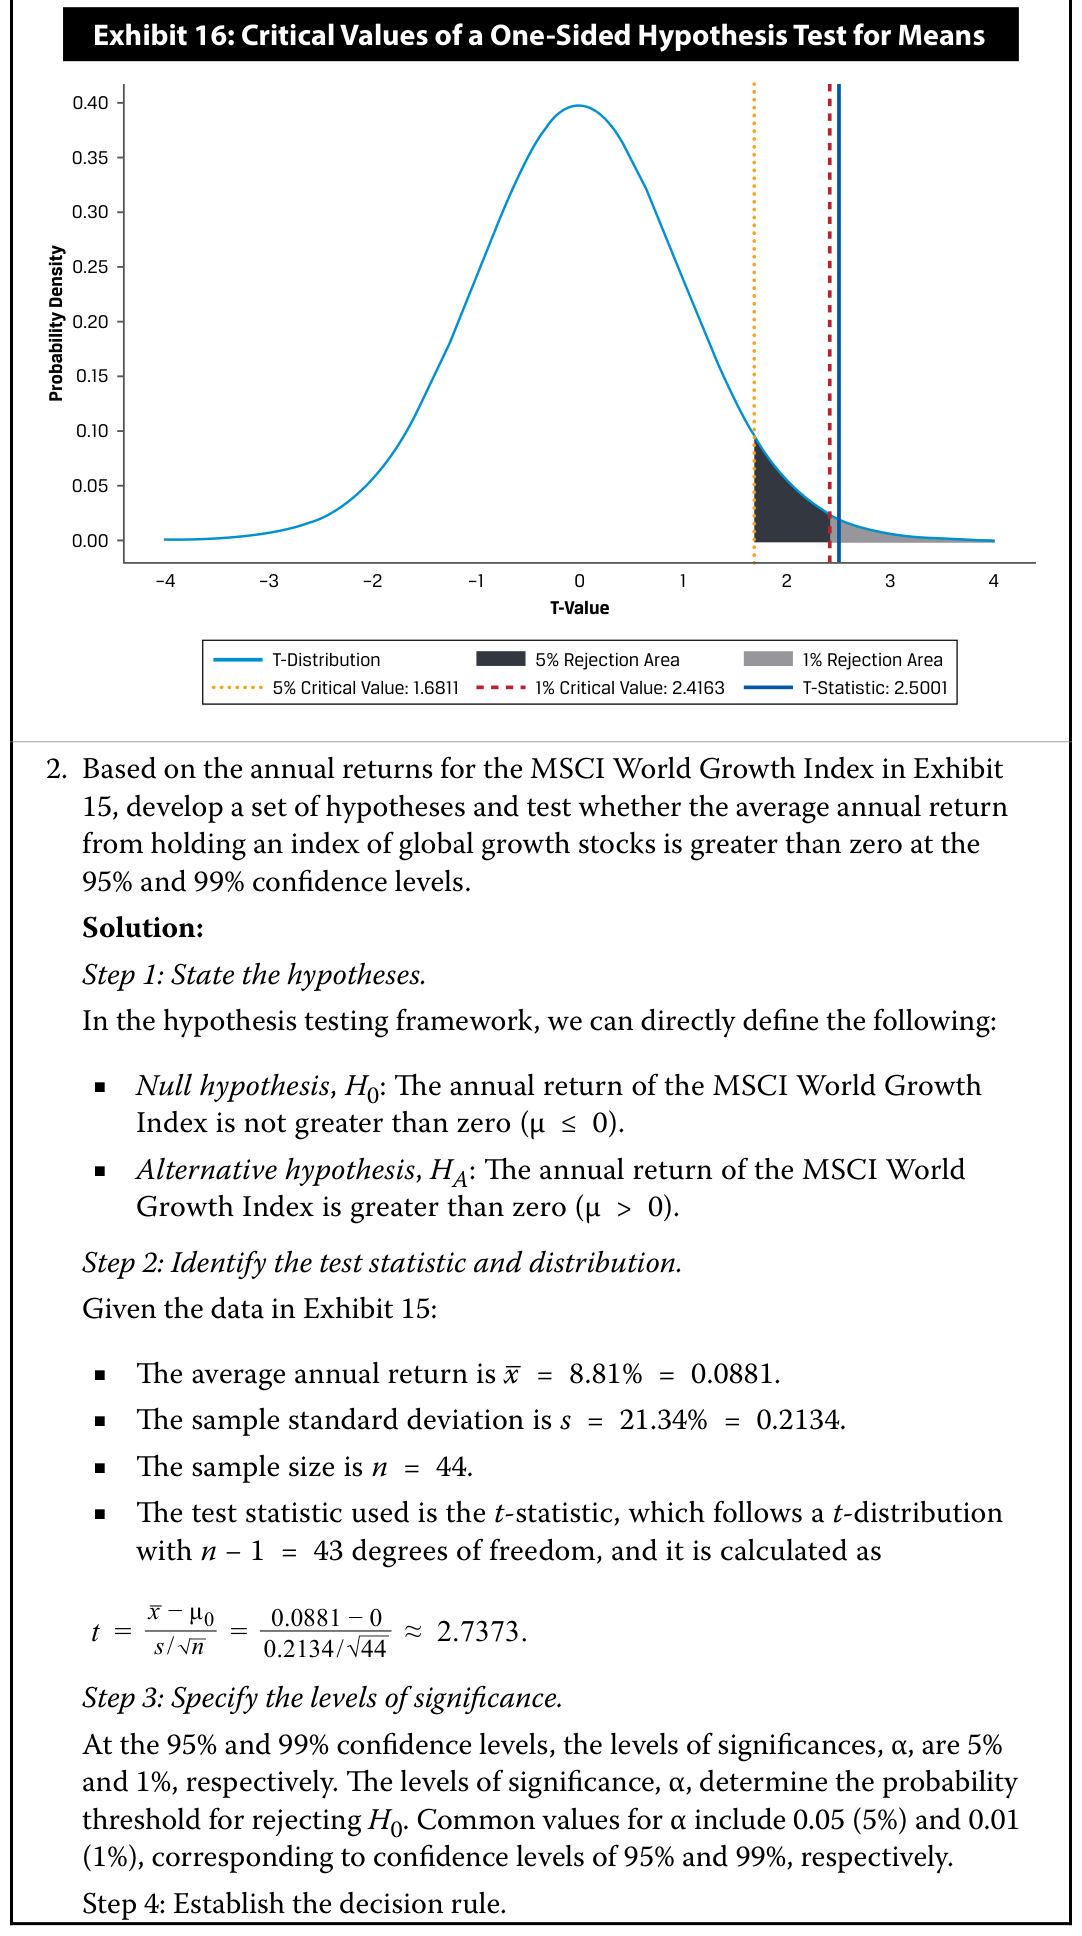
\includegraphics[width=0.75\linewidth]{002_figs/007_Module_7/exhibit_16.png}
	\caption{One-Sided Mean Test Critical Values and Rejection Regions}
	\label{fig:mod7_exhibit_16}
\end{figure}
% Reference: CFA Curriculum 2027, Volume 1, Module 7, Page 348, Exhibit 16

\begin{tcolorbox}[
	colback=gray!5!white,
	colframe=black!15!white,
	boxrule=0.5pt,
	arc=3pt,
	title=\textbf{Case Study: Testing MSCI World Growth Index Mean Return},
	coltitle=black,
	colbacktitle=black!5!white,
	before skip=6pt,
	after skip=6pt,
	breakable
]
We test whether the average return of global growth stocks is different from zero ($H_0: \mu = 0$ vs $H_A: \mu \ne 0$).
\begin{enumerate}
	\item \textbf{Calculate Test Statistic:} $t = \frac{0.0881 - 0}{0.2134 / \sqrt{44}} \approx 2.7373$.
	\item \textbf{Decision Rule ($df = 43$):} Two-tailed critical values are $\pm 2.0167$ (at 5\%) and $\pm 2.6951$ (at 1\%) (Exhibit~\ref{fig:mod7_exhibit_17}).
	\item \textbf{Conclusion:} Since $2.7373 > 2.6951$, we reject $H_0$ at both levels. Growth stock returns are significantly different from zero.
\end{enumerate}
\end{tcolorbox}

\begin{figure}[!htbp]
	\centering
	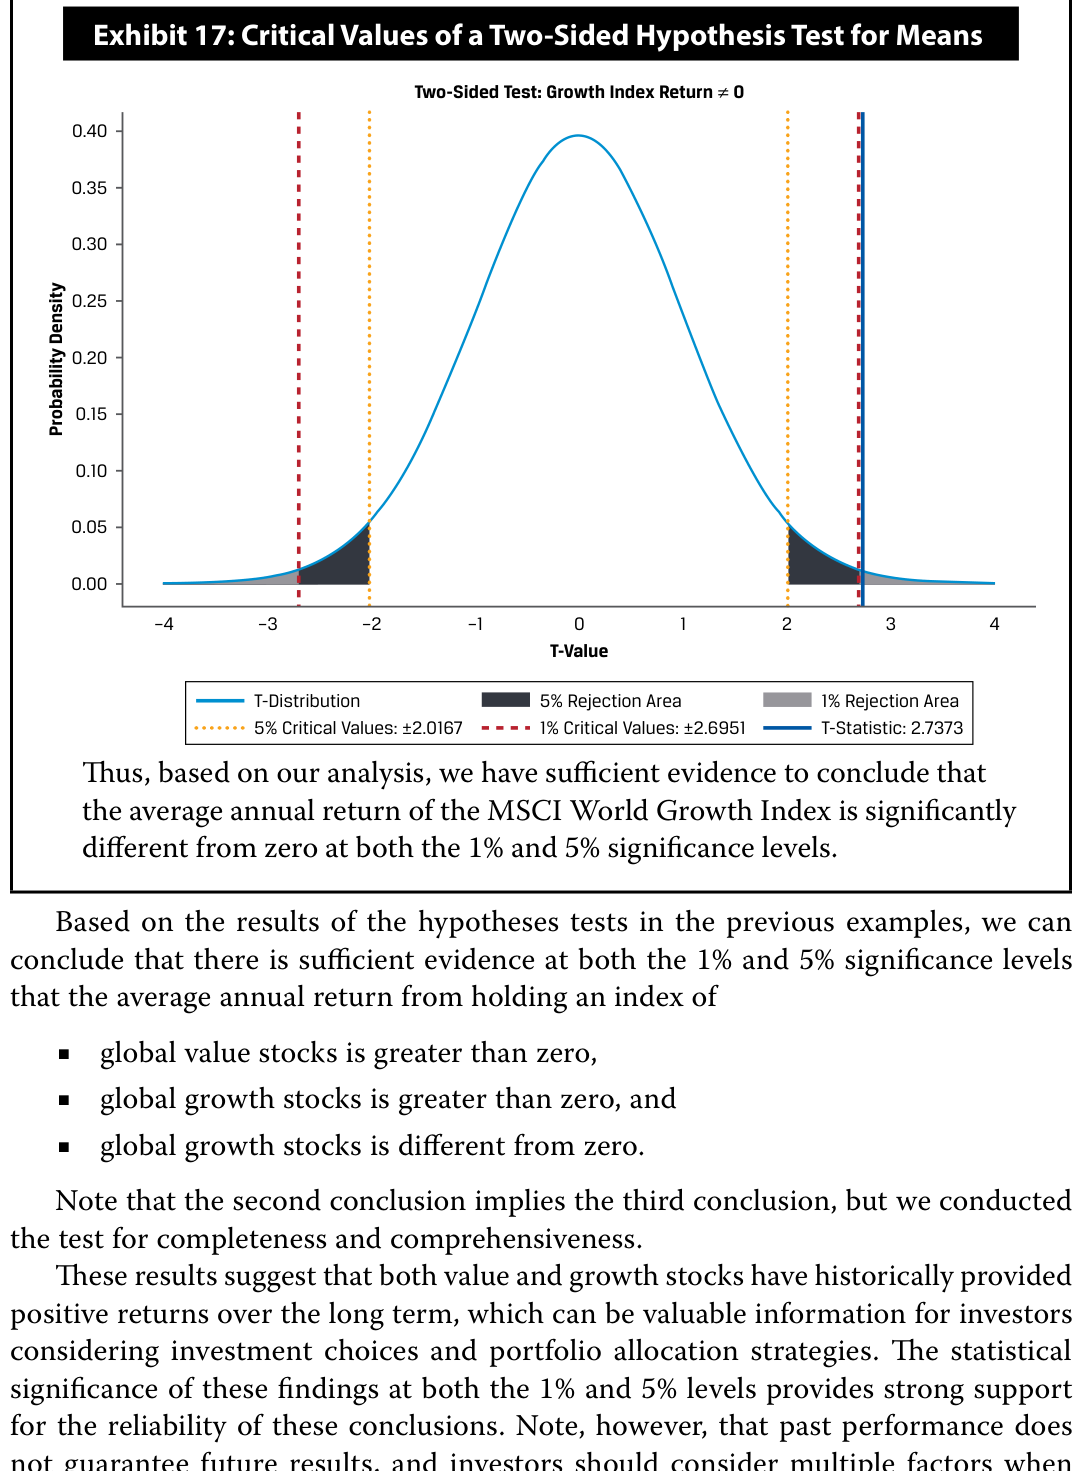
\includegraphics[width=0.75\linewidth]{002_figs/007_Module_7/exhibit_17.png}
	\caption{Two-Sided Mean Test Critical Values and Rejection Regions}
	\label{fig:mod7_exhibit_17}
\end{figure}
% Reference: CFA Curriculum 2027, Volume 1, Module 7, Page 350, Exhibit 17

\subsubsection{Test of a Single Variance}
To test the variance of a single normally distributed population, we use the Chi-square ($\chi^2$) test statistic with $n - 1$ degrees of freedom (Exhibit~\ref{fig:mod7_exhibit_18}):
\begin{equation}
	\chi^2 = \frac{(n-1)s^2}{\sigma_0^2}
	\label{eq:single_variance_chisq_m7}
\end{equation}
% Reference: CFA Curriculum 2027, Volume 1, Module 7, Page 351, Equation (7)

\begin{figure}[!htbp]
	\centering
	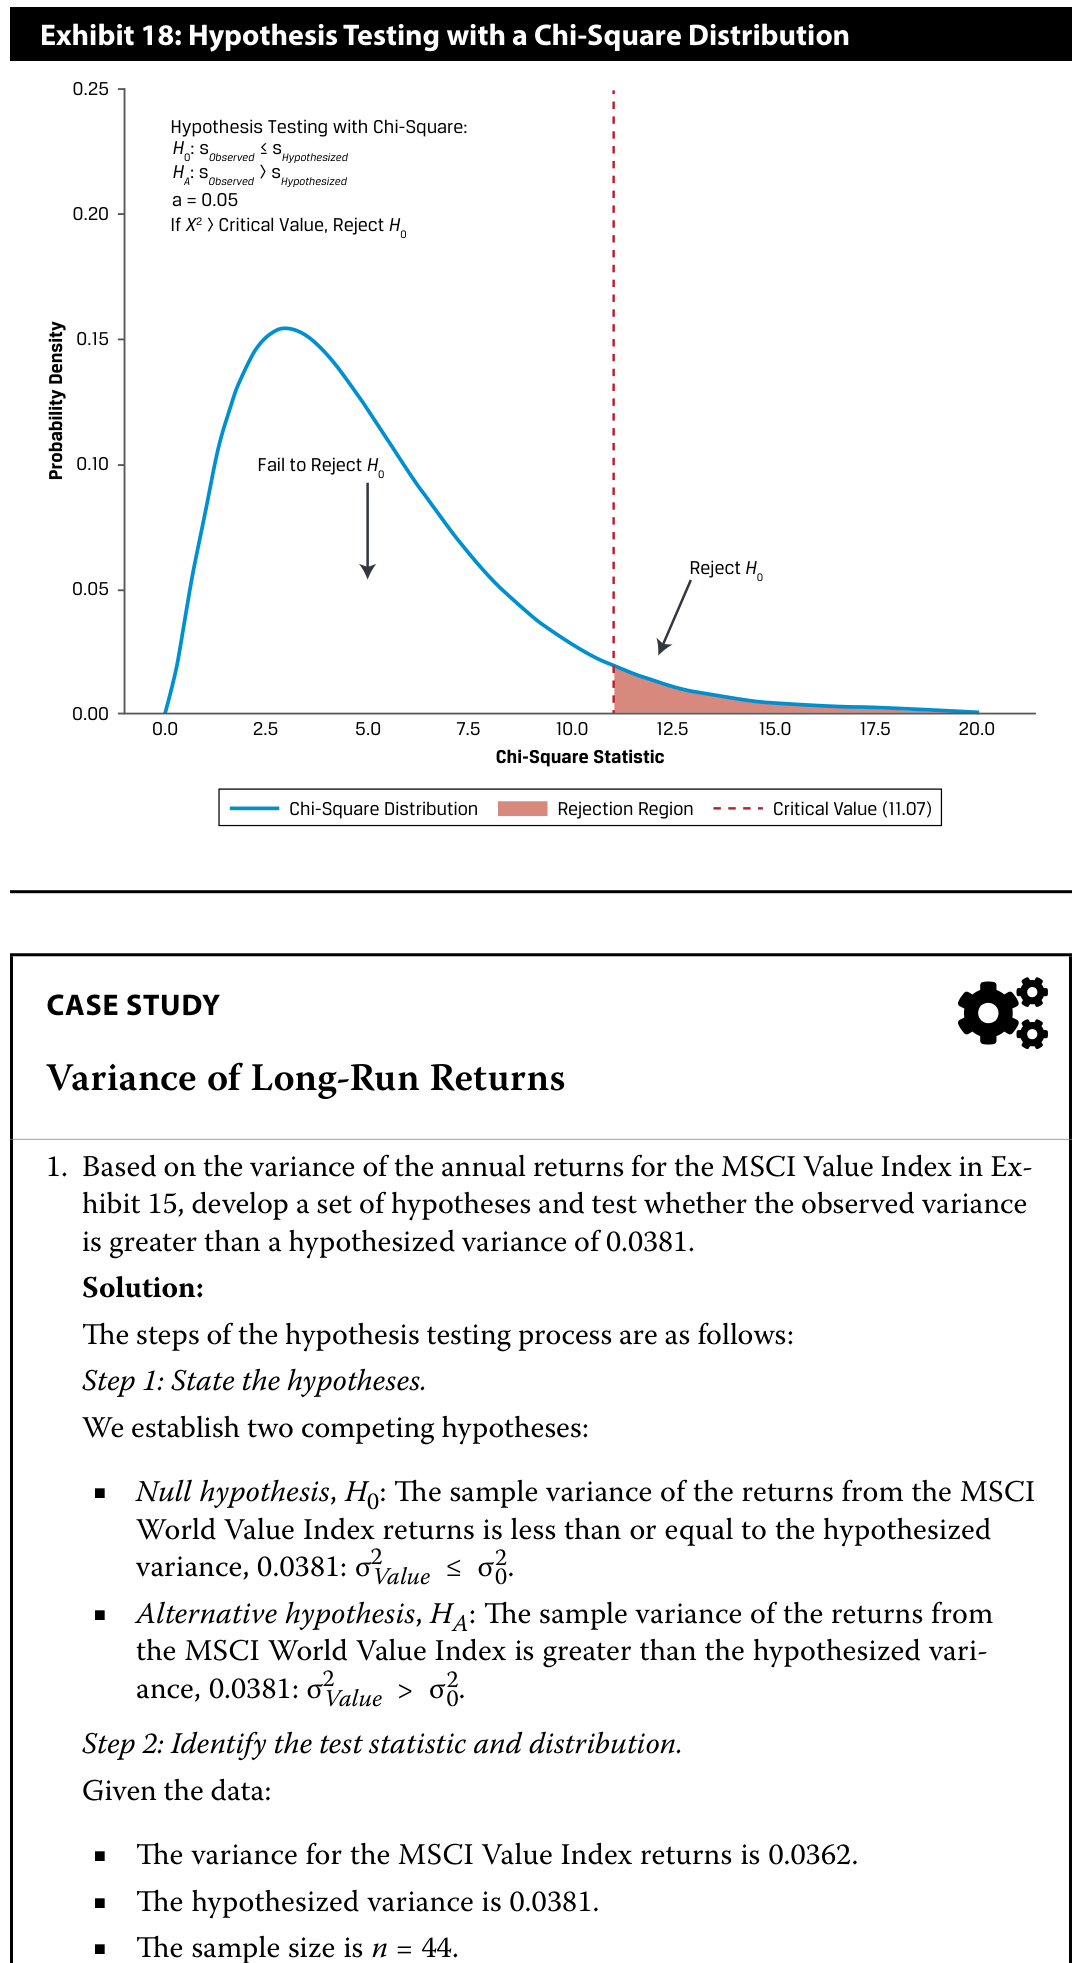
\includegraphics[width=0.75\linewidth]{002_figs/007_Module_7/exhibit_18.png}
	\caption{Hypothesis Testing with a Chi-Square Distribution ($df=5$)}
	\label{fig:mod7_exhibit_18}
\end{figure}
% Reference: CFA Curriculum 2027, Volume 1, Module 7, Page 352, Exhibit 18

\begin{tcolorbox}[
	colback=gray!5!white,
	colframe=black!15!white,
	boxrule=0.5pt,
	arc=3pt,
	title=\textbf{Case Study: Testing MSCI Value Index Variance},
	coltitle=black,
	colbacktitle=black!5!white,
	before skip=6pt,
	after skip=6pt,
	breakable
]
We test whether the variance of the Value Index is greater than $0.0381$ ($H_0: \sigma^2 \le 0.0381$ vs $H_A: \sigma^2 > 0.0381$).
\begin{enumerate}
	\item \textbf{Calculate Test Statistic ($df = 43$):} $\chi^2 = \frac{43 \times 0.0362}{0.0381} \approx 40.8237$.
	\item \textbf{Decision Rule:} Right-tailed critical values are $\chi^2_{0.05} = 59.3035$ and $\chi^2_{0.01} = 67.4593$ (Exhibit~\ref{fig:mod7_exhibit_19}).
	\item \textbf{Conclusion:} Since $40.8237 < 59.3035$, we fail to reject $H_0$. The variance is not significantly greater than $0.0381$.
\end{enumerate}
\end{tcolorbox}

\begin{figure}[!htbp]
	\centering
	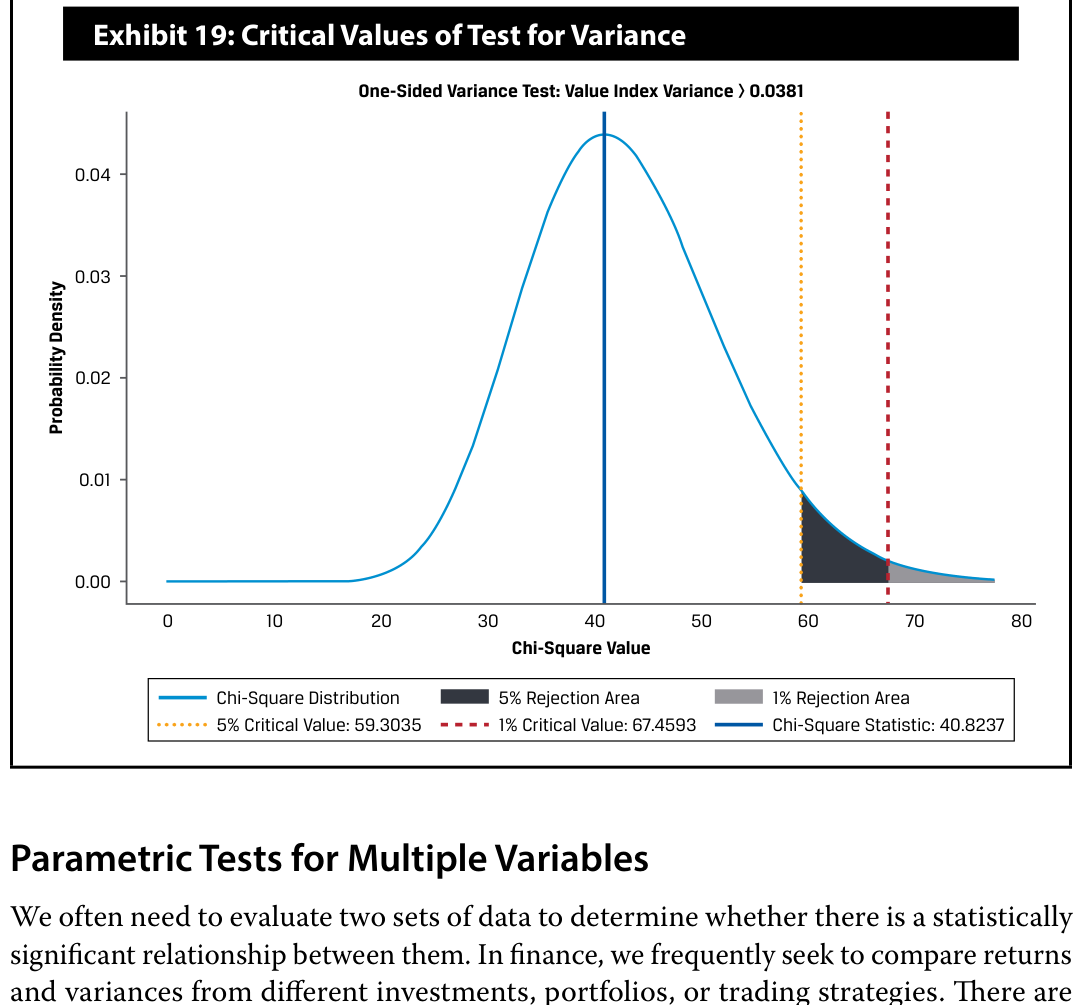
\includegraphics[width=0.75\linewidth]{002_figs/007_Module_7/exhibit_19.png}
	\caption{One-Sided Variance Test Critical Values and Rejection Regions}
	\label{fig:mod7_exhibit_19}
\end{figure}
% Reference: CFA Curriculum 2027, Volume 1, Module 7, Page 353, Exhibit 19

\subsection{Parametric Tests for Multiple Variables}
We compare the means and variances of two populations.

\subsubsection{Test of Equality of Two Unknown Means (Independent Samples)}
Assuming equal population variances, the $t$-test statistic with $n_1 + n_2 - 2$ degrees of freedom is:
\begin{equation}
	t = \frac{(\bar{X}_1 - \bar{X}_2) - \Delta_0}{\sqrt{\frac{s_p^2}{n_1} + \frac{s_p^2}{n_2}}} \quad \text{where} \quad s_p^2 = \frac{(n_1-1)s_1^2 + (n_2-1)s_2^2}{n_1+n_2-2}
	\label{eq:indep_means_t_test_m7}
\end{equation}
% Reference: CFA Curriculum 2027, Volume 1, Module 7, Page 354, Equation (8)

\begin{tcolorbox}[
	colback=gray!5!white,
	colframe=black!15!white,
	boxrule=0.5pt,
	arc=3pt,
	title=\textbf{Case Study: Comparing Growth vs Value Average Returns},
	coltitle=black,
	colbacktitle=black!5!white,
	before skip=6pt,
	after skip=6pt,
	breakable
]
We test whether Growth average returns exceed Value returns ($H_0: \mu_G - \mu_V \le 0$ vs $H_A: \mu_G - \mu_V > 0$).
\begin{enumerate}
	\item \textbf{Calculate Test Statistic ($df = 86$):}
	      \[ t = \frac{0.0881 - 0.0717 - 0}{\sqrt{\frac{0.0456}{44} + \frac{0.0362}{44}}} = \frac{0.0164}{0.0431} \approx 0.3805 \]
	\item \textbf{Decision Rule:} One-tailed critical values are $t_{0.05} = 1.6628$ and $t_{0.01} = 2.3705$ (Exhibit~\ref{fig:mod7_exhibit_20}).
	\item \textbf{Conclusion:} Since $0.3805 < 1.6628$, we fail to reject $H_0$. The difference in average returns is not statistically significant.
\end{enumerate}
\end{tcolorbox}

\begin{figure}[!htbp]
	\centering
	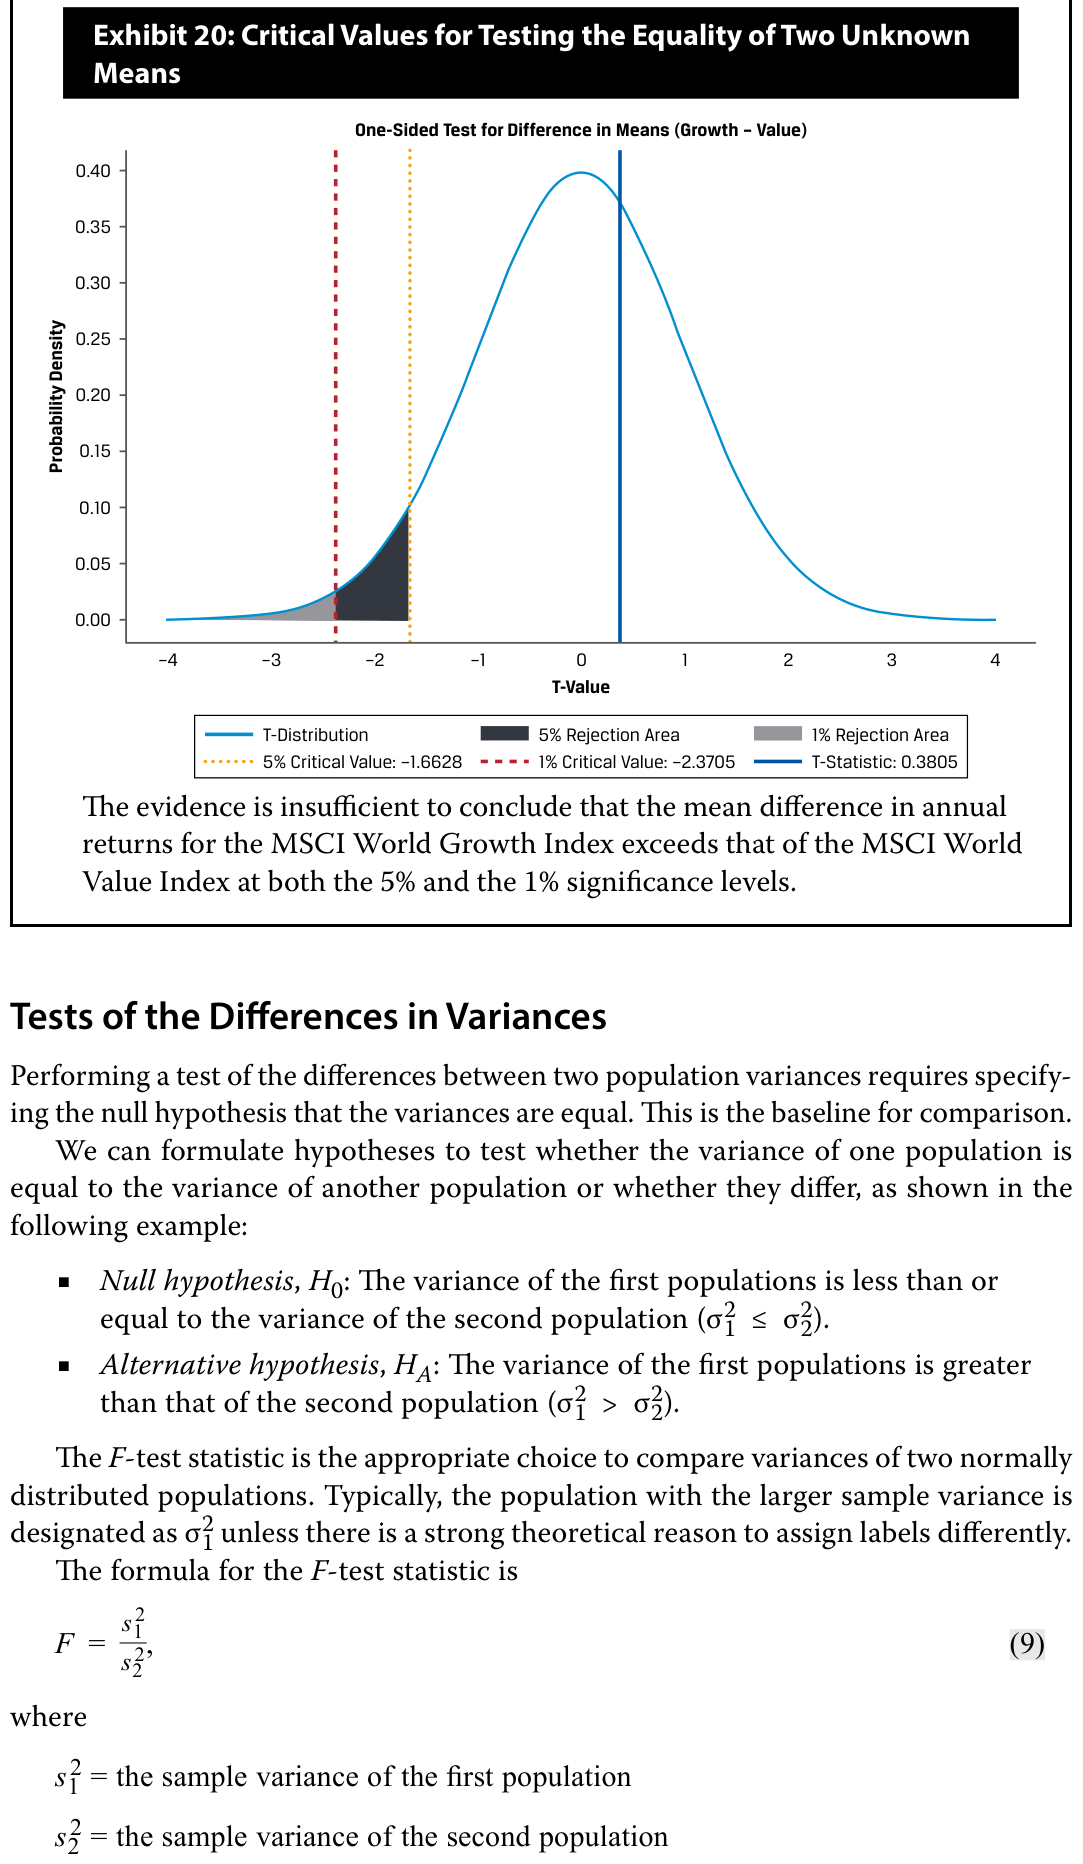
\includegraphics[width=0.75\linewidth]{002_figs/007_Module_7/exhibit_20.png}
	\caption{Independent Means Test Critical Values and Rejection Regions}
	\label{fig:mod7_exhibit_20}
\end{figure}
% Reference: CFA Curriculum 2027, Volume 1, Module 7, Page 356, Exhibit 20

\subsubsection{Test of Difference in Two Variances ($F$-test)}
To compare variances of two independent, normally distributed populations, the $F$-test statistic is:
\begin{equation}
	F = \frac{s_1^2}{s_2^2} \quad (\text{where } s_1^2 \ge s_2^2)
	\label{eq:variance_ratio_f_test_m7}
\end{equation}
% Reference: CFA Curriculum 2027, Volume 1, Module 7, Page 356, Equation (9)
With $df_1 = n_1 - 1$ and $df_2 = n_2 - 1$ (Exhibit~\ref{fig:mod7_exhibit_21}).

\begin{figure}[!htbp]
	\centering
	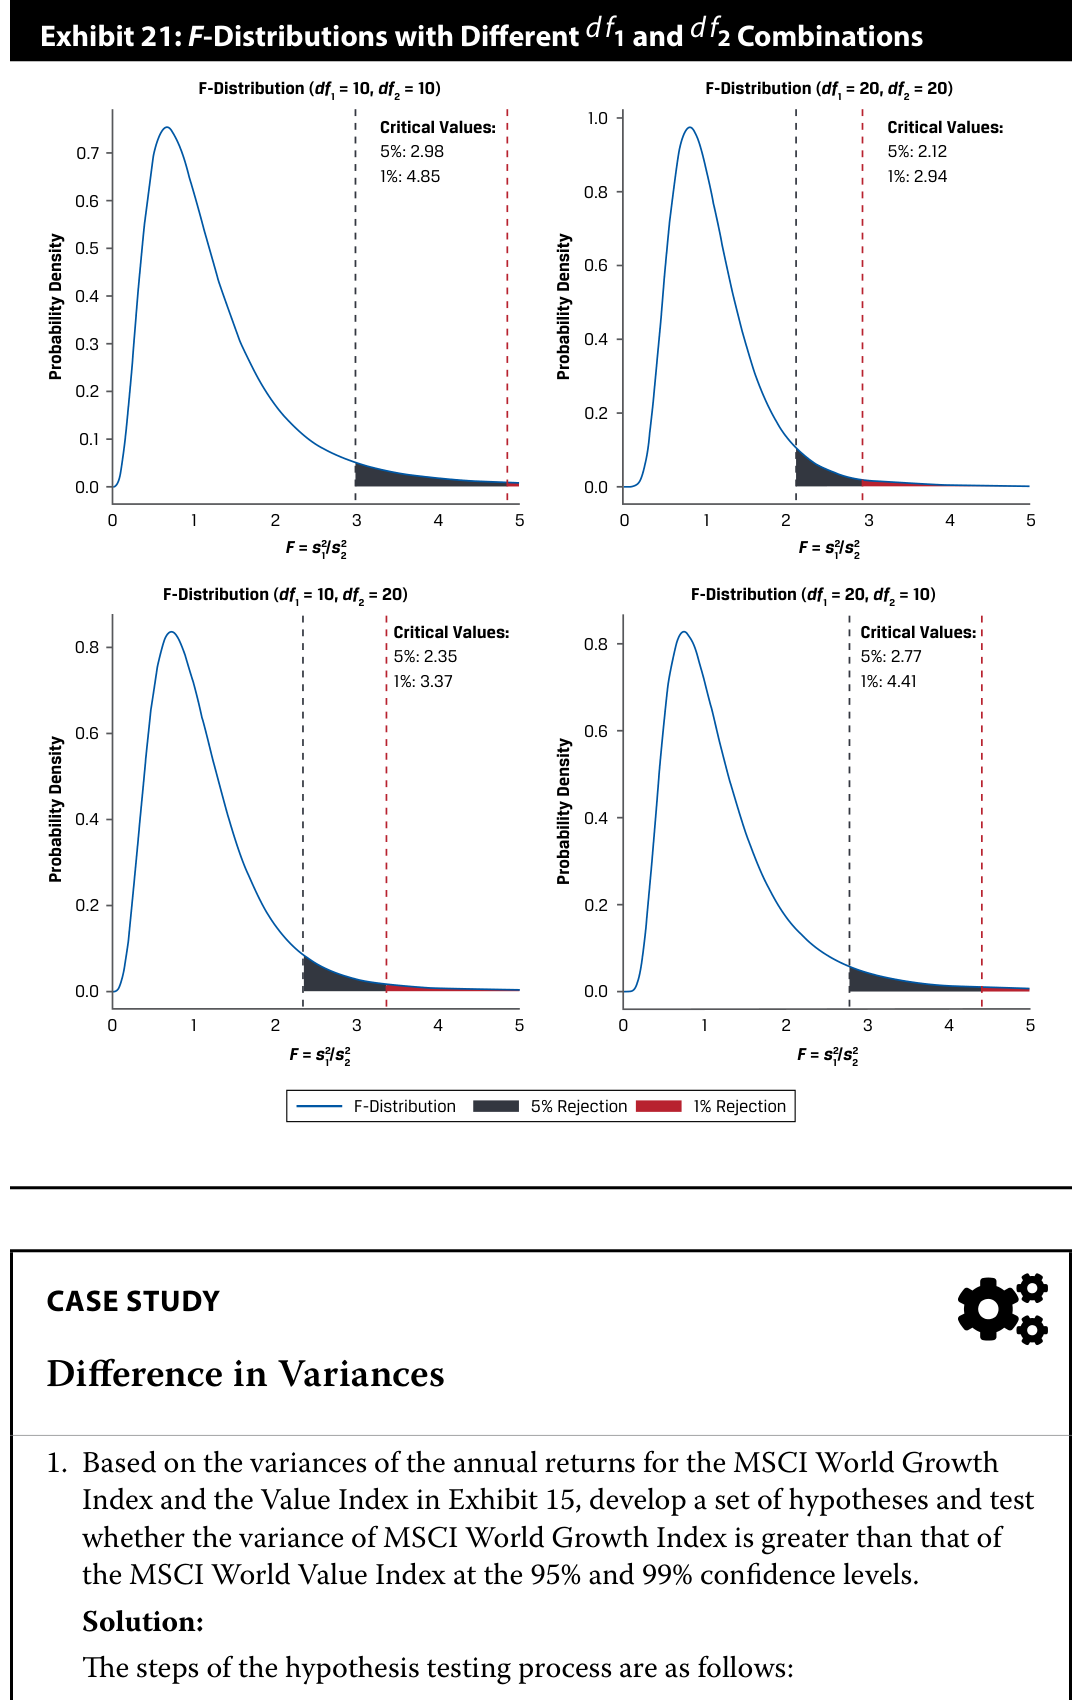
\includegraphics[width=0.85\linewidth]{002_figs/007_Module_7/exhibit_21.png}
	\caption{$F$-Distributions with Different Degrees of Freedom}
	\label{fig:mod7_exhibit_21}
\end{figure}
% Reference: CFA Curriculum 2027, Volume 1, Module 7, Page 357, Exhibit 21

\begin{tcolorbox}[
	colback=gray!5!white,
	colframe=black!15!white,
	boxrule=0.5pt,
	arc=3pt,
	title=\textbf{Case Study: Comparing Growth vs Value Variances},
	coltitle=black,
	colbacktitle=black!5!white,
	before skip=6pt,
	after skip=6pt,
	breakable
]
We test whether Growth variance is greater than Value variance ($H_0: \sigma_G^2 \le \sigma_V^2$ vs $H_A: \sigma_G^2 > \sigma_V^2$).
\begin{enumerate}
	\item \textbf{Calculate Test Statistic ($df_1 = 43, df_2 = 43$):} $F = \frac{0.0456}{0.0362} \approx 1.2595$.
	\item \textbf{Decision Rule:} Critical values are $F_{0.05} = 1.6607$ and $F_{0.01} = 2.0569$ (Exhibit~\ref{fig:mod7_exhibit_22}).
	\item \textbf{Conclusion:} Since $1.2595 < 1.6607$, we fail to reject $H_0$. Growth variance is not significantly larger.
\end{enumerate}
\end{tcolorbox}


\begin{figure}[!htbp]
	\centering
	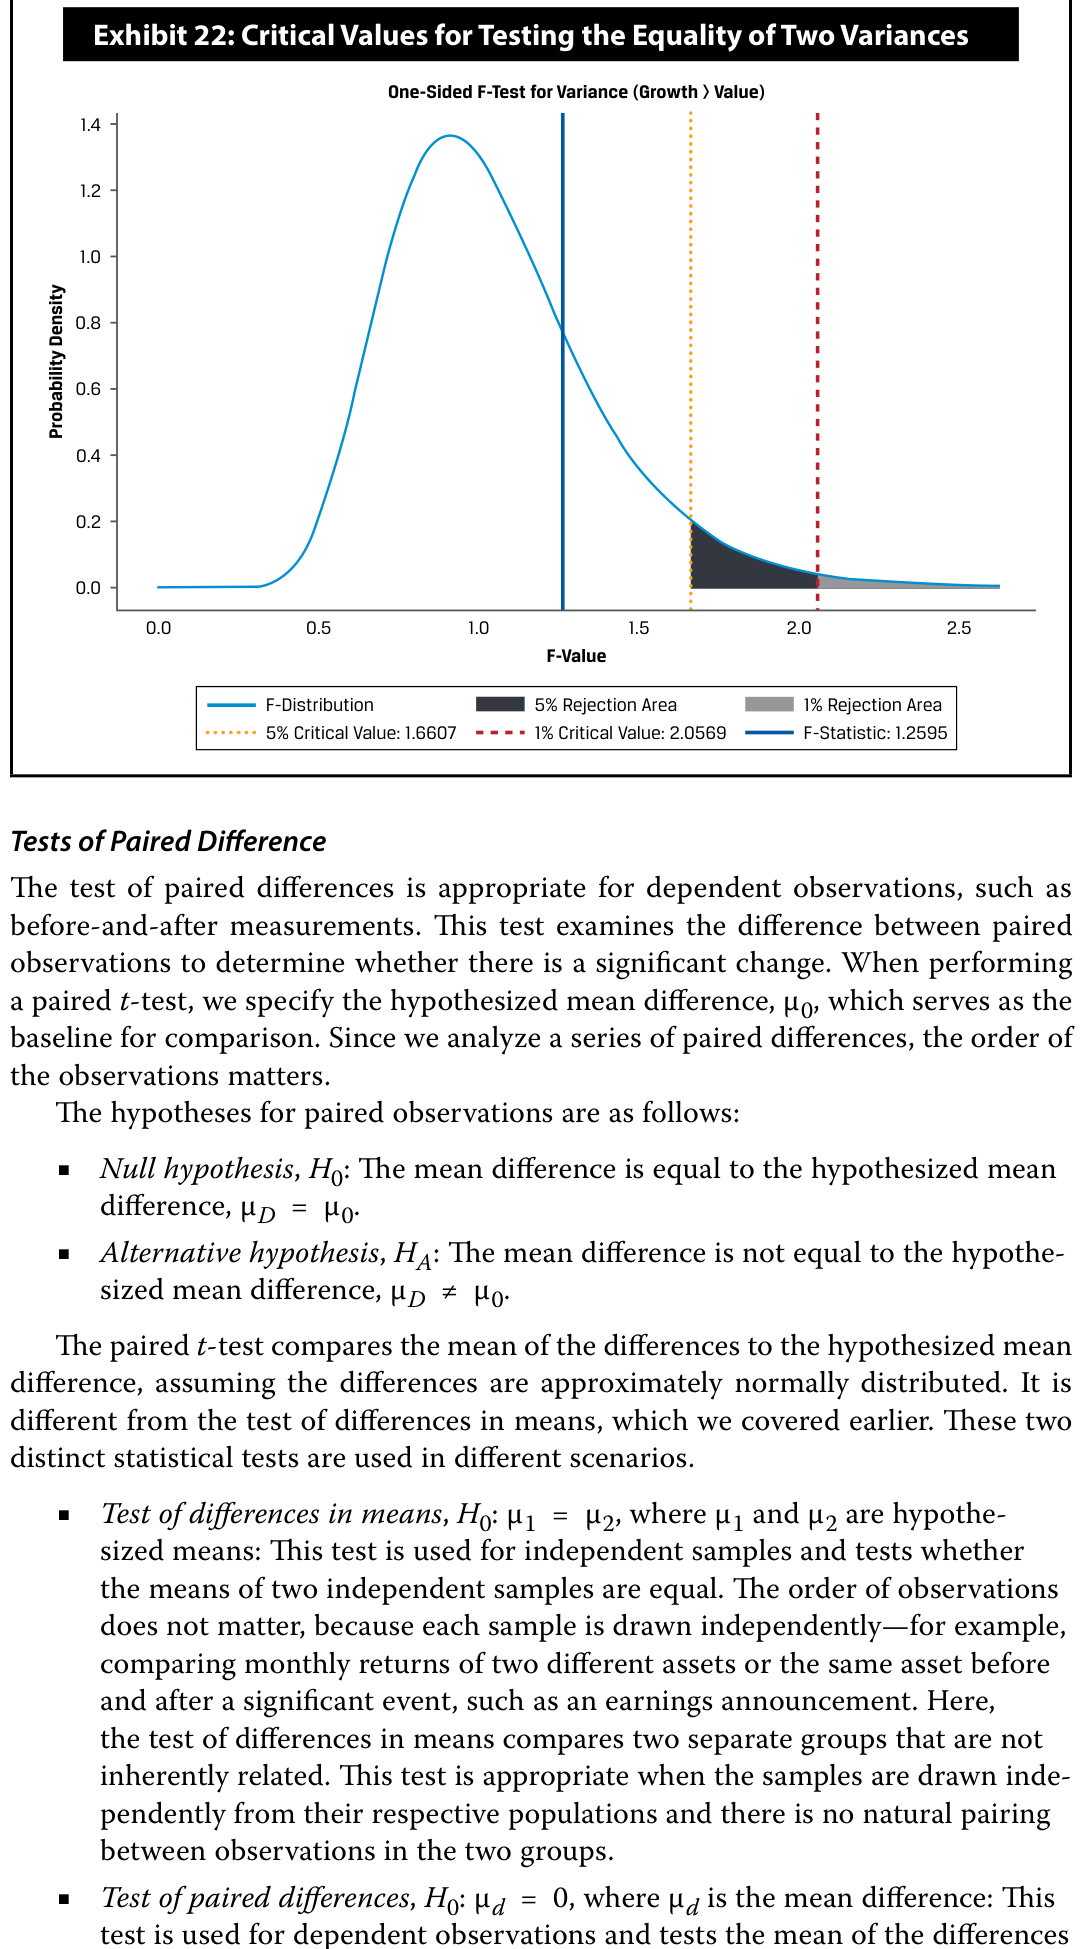
\includegraphics[width=0.75\linewidth]{002_figs/007_Module_7/exhibit_22.png}
	\caption{Equality of Variances $F$-Test Critical Values}
	\label{fig:mod7_exhibit_22}
\end{figure}
% Reference: CFA Curriculum 2027, Volume 1, Module 7, Page 359, Exhibit 22

\subsubsection{Test of Paired Differences (Dependent Samples)}
For dependent observations, the $t$-test statistic with $n - 1$ degrees of freedom is:
\begin{equation}
	t = \frac{\bar{d} - \mu_{d0}}{s_d / \sqrt{n}}
	\label{eq:paired_means_t_test_m7}
\end{equation}
% Reference: CFA Curriculum 2027, Volume 1, Module 7, Page 360, Equation (10)
Where $\bar{d}$ is the sample mean difference, and $s_d$ is the sample standard deviation of differences.

\begin{tcolorbox}[
	colback=gray!5!white,
	colframe=black!15!white,
	boxrule=0.5pt,
	arc=3pt,
	title=\textbf{Case Study: Paired Difference of Growth and Value Returns},
	coltitle=black,
	colbacktitle=black!5!white,
	before skip=6pt,
	after skip=6pt,
	breakable
]
We test whether the mean difference in paired returns is different from zero ($H_0: \mu_d = 0$ vs $H_A: \mu_d \ne 0$). We calculate $\bar{d} = 1.64\%$ and $s_d = 10.62\%$.
\begin{enumerate}
	\item \textbf{Calculate Test Statistic ($df = 43$):} $t = \frac{0.0164 - 0}{0.1062 / \sqrt{44}} \approx 1.0243$.
	\item \textbf{Decision Rule:} Two-tailed critical values are $\pm 2.0167$ (at 5\% significance, Exhibit~\ref{fig:mod7_exhibit_23}).
	\item \textbf{Conclusion:} Since $1.0243 < 2.0167$, we fail to reject $H_0$. The paired differences are not statistically significant.
\end{enumerate}
\end{tcolorbox}

\begin{figure}[!htbp]
	\centering
	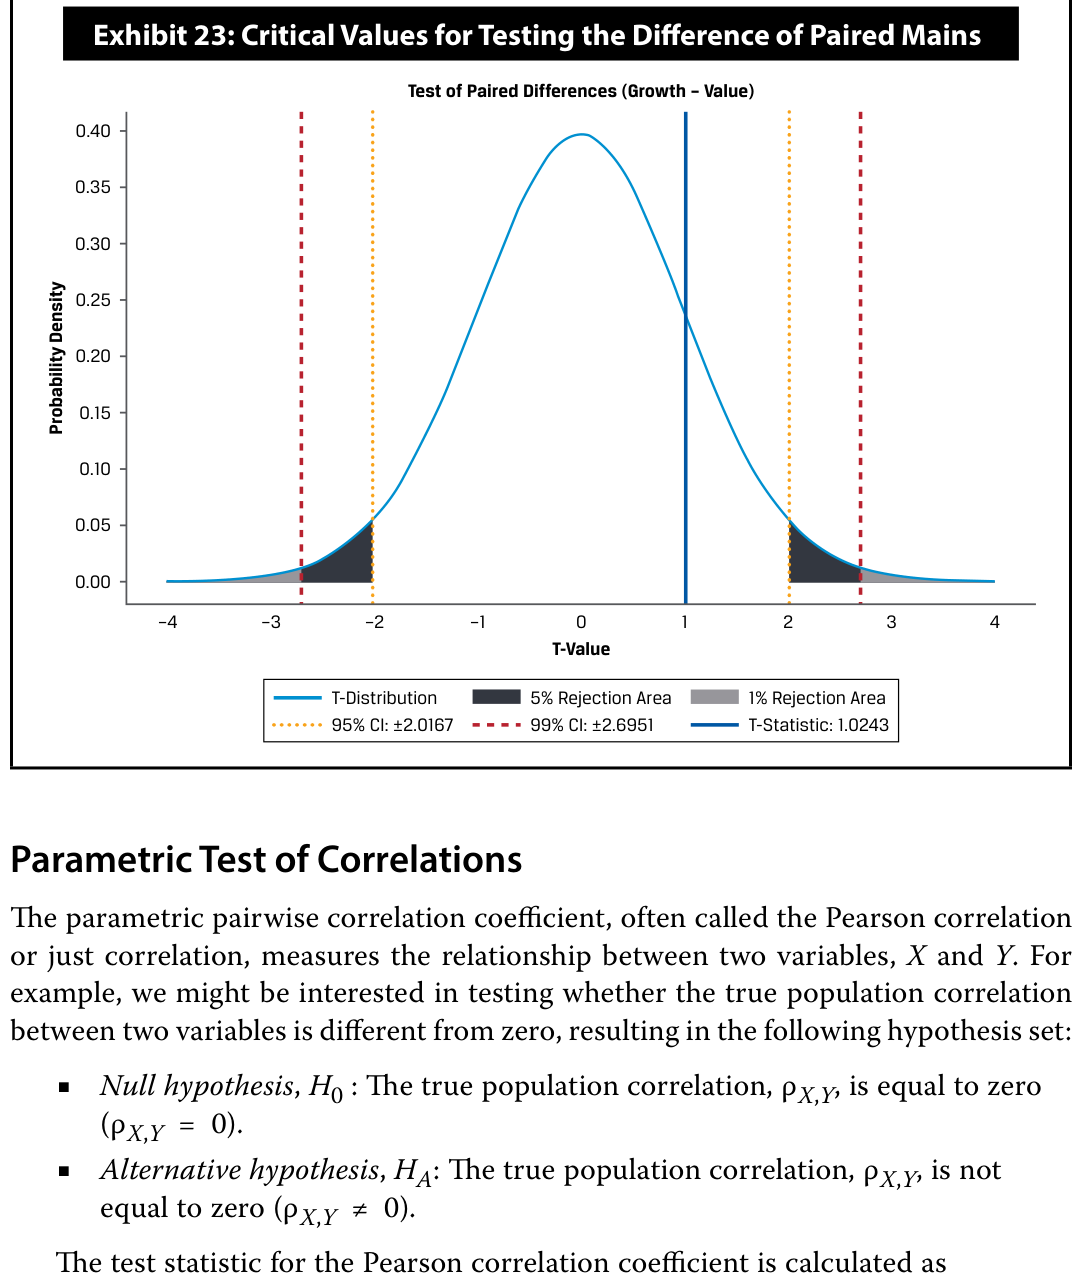
\includegraphics[width=0.75\linewidth]{002_figs/007_Module_7/exhibit_23.png}
	\caption{Paired Means Test Critical Values and Rejection Regions}
	\label{fig:mod7_exhibit_23}
\end{figure}
% Reference: CFA Curriculum 2027, Volume 1, Module 7, Page 361, Exhibit 23

\subsubsection{Parametric Test of Correlations}
To test whether the Pearson correlation coefficient between $X$ and $Y$ is zero ($H_0: \rho = 0$ vs $H_A: \rho \ne 0$), we use the $t$-test statistic with $n - 2$ degrees of freedom:
\begin{equation}
	t = \frac{r \sqrt{n-2}}{\sqrt{1 - r^2}}
	\label{eq:correlation_t_test_m7}
\end{equation}
% Reference: CFA Curriculum 2027, Volume 1, Module 7, Page 361, Equation (11)

As sample size $n$ increases, the standard error decreases, causing the power of the test to increase. Thus, in very large datasets, even minor correlations are rejected as statistically different from zero (Exhibit~\ref{fig:mod7_exhibit_24}).

\begin{figure}[!htbp]
	\centering
	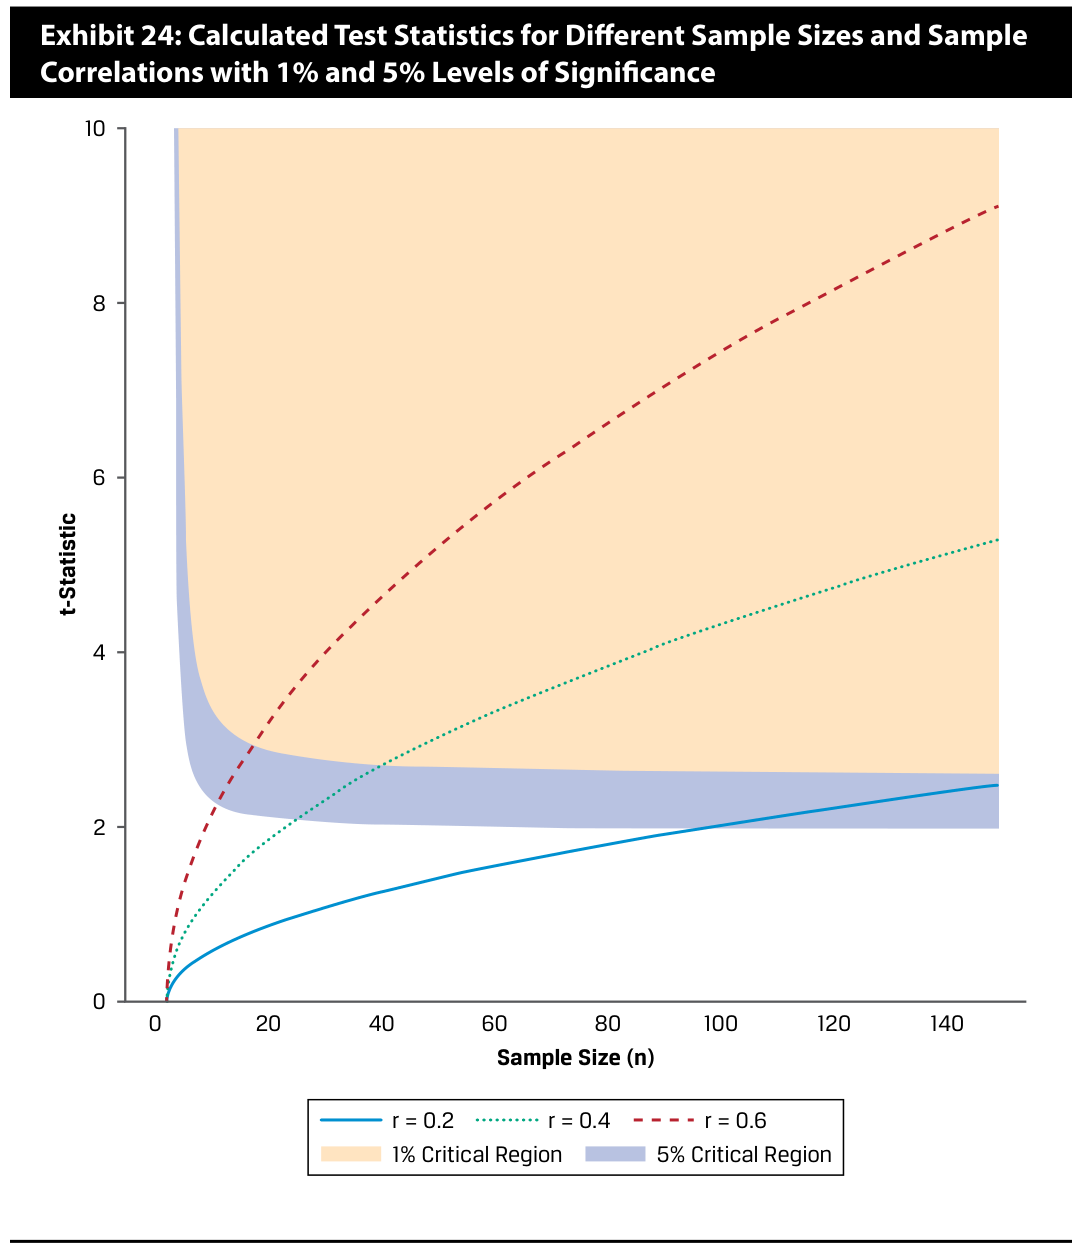
\includegraphics[width=0.75\linewidth]{002_figs/007_Module_7/exhibit_24.png}
	\caption{t-Statistic Values for Various Sample Sizes and Correlation Coefficients}
	\label{fig:mod7_exhibit_24}
\end{figure}
% Reference: CFA Curriculum 2027, Volume 1, Module 7, Page 362, Exhibit 24

\begin{tcolorbox}[
	colback=gray!5!white,
	colframe=black!15!white,
	boxrule=0.5pt,
	arc=3pt,
	title=\textbf{Case Study: Fund Correlations and STOXX50 Index},
	coltitle=black,
	colbacktitle=black!5!white,
	before skip=6pt,
	after skip=6pt,
	breakable
]
Table~\ref{tab:fund_correlations_m7} presents correlations of four funds with the STOXX50 index ($n = 36$, $df = 34$). The critical t-value at the 5\% significance level is $\pm 2.032$.
For Fund 3 and Fund 4:
\[ t = \frac{0.3102\sqrt{34}}{\sqrt{1 - 0.3102^2}} \approx 1.903 \]
Since $1.903 < 2.032$, the correlation between Fund 3 and Fund 4 is not statistically significant. However, all other correlations (e.g., Fund 2 and STOXX50, $r=0.8223 \implies t=8.426$) are statistically significant, suggesting limited diversification benefits except between Fund 3 and 4.
\end{tcolorbox}

\begin{table}[!htbp]
\centering
\caption{Fund Correlations Matrix ($n=36$)}
\label{tab:fund_correlations_m7}
\begin{tabular}{p{0.15\linewidth} p{0.14\linewidth} p{0.14\linewidth} p{0.14\linewidth} p{0.14\linewidth} p{0.14\linewidth}}
\toprule
\textbf{Asset} & \textbf{Fund 1} & \textbf{Fund 2} & \textbf{Fund 3} & \textbf{Fund 4} & \textbf{STOXX50} \\
\midrule
\textbf{Fund 1} & 1.0000 & --- & --- & --- & --- \\
\textbf{Fund 2} & 0.9231 & 1.0000 & --- & --- & --- \\
\textbf{Fund 3} & 0.4771 & 0.4156 & 1.0000 & --- & --- \\
\textbf{Fund 4} & 0.7111 & 0.7238 & 0.3102 & 1.0000 & --- \\
\textbf{STOXX50} & 0.8277 & 0.8223 & 0.5791 & 0.7515 & 1.0000 \\
\bottomrule
\end{tabular}
\end{table}
% Reference: CFA Curriculum 2027, Volume 1, Module 7, Page 363

\subsection{P-Value and P-Hacking}
The p-value is the smallest level of significance at which we reject the null hypothesis:
\begin{itemize}
	\item \textbf{Decision Rule:} Reject $H_0$ if $p\text{-value} < \alpha$; otherwise, fail to reject.
\end{itemize}
For the MSCI Value Index mean test ($t = 2.5001$, $df = 43$), the one-tailed $p$-value is $0.0081$, which is less than both $5\%$ and $1\%$, leading to rejection of $H_0$.

\begin{examtip}
\textbf{Beware of P-Hacking}\\
p-hacking refers to the practice of manipulating data or models (such as trimming time horizons, selectively removing outliers, or testing dozens of models) until a statistically significant result ($p < 0.05$) is obtained. This inflates the Type I error rate. To prevent p-hacking, analysts must use out-of-sample validation and strict methodologies.
\end{examtip}

\subsection{Practical Implementation (Excel and Google Sheets)}
Table~\ref{tab:excel_functions_m7} lists functions to compute critical values for hypothesis testing.

\begin{table}[!htbp]
\centering
\caption{Built-In Excel and Google Sheet Functions for Hypothesis Testing}
\label{tab:excel_functions_m7}
\begin{tabular}{p{0.22\linewidth} | p{0.34\linewidth} | p{0.34\linewidth}}
\toprule
\textbf{Function} & \textbf{Excel Formula} & \textbf{Google Sheets Formula} \\
\midrule
Inverse Student's t & \texttt{=T.INV(prob, df)} & \texttt{=T.INV(prob, df)} \\
Two-tailed t Inverse & \texttt{=T.INV.2T(prob, df)} & \texttt{=T.INV.2T(prob, df)} \\
Right-tailed t Dist & \texttt{=T.DIST.RT(x, df)} & \texttt{=T.DIST.RT(x, df)} \\
Inverse Standard Normal & \texttt{=NORM.S.INV(prob)} & \texttt{=NORM.S.INV(prob)} \\
Inverse Normal Cumulative & \texttt{=NORM.INV(prob, mean, sd)} & \texttt{=NORM.INV(prob, mean, sd)} \\
Inverse Chi-Square & \texttt{=CHISQ.INV.RT(prob, df)} & \texttt{=CHISQ.INV.RT(prob, df)} \\
Inverse Left-tail F & \texttt{=F.INV(prob, df1, df2)} & \texttt{=F.INV(prob, df1, df2)} \\
Inverse Right-tail F & \texttt{=F.INV.RT(prob, df1, df2)} & \texttt{=F.INV.RT(prob, df1, df2)} \\
\bottomrule
\end{tabular}
\end{table}
% Reference: CFA Curriculum 2027, Volume 1, Module 7, Page 366, Exhibit 25

\section{NON-PARAMETRIC TESTS}
\begin{center}
\begin{tabular}{p{0.06\linewidth} | p{0.88\linewidth}}
	c & compare and contrast parametric and non-parametric tests, describe situations in which each is the more appropriate type of test, construct appropriate hypothesis tests, and interpret the results \\
\end{tabular}
\end{center}

\textcolor{blue}{\textit{Thực tế: Khi dữ liệu không chuẩn (đuôi béo, lệch) hoặc ở dạng định danh/thứ bậc, kiểm định phi tham số (Non-parametric) như Spearman hoặc Chi-square test of independence là bắt buộc để tránh kết luận sai lệch.}}

\subsection{Comparison of Parametric and Non-Parametric Tests}
\begin{itemize}
	\item \textbf{Parametric Tests:} Perform testing using parameters (mean, variance) and require specific distribution assumptions (e.g., normality). They are more powerful if assumptions are met.
	\item \textbf{Non-Parametric Tests:} Do not make distribution assumptions. They are suitable for ordinal/categorical data, small sample sizes, or when outliers skew parametric estimations. However, they are less powerful when normality assumptions hold.
\end{itemize}

\subsection{Non-Parametric Test for Correlation (Spearman Rank Correlation)}
The Spearman rank correlation coefficient ($r_s$) evaluates monotonic (not necessarily linear) relationships by analyzing the ranks of variables:
\begin{equation}
	r_s = 1 - \frac{6 \sum_{i=1}^n d_i^2}{n(n^2 - 1)}
	\label{eq:spearman_formula_m7}
\end{equation}
% Reference: CFA Curriculum 2027, Volume 1, Module 7, Page 370
Where $d_i$ is the difference in ranks for each observation pair. For $n > 30$, the test statistic follows a $t$-distribution with $n - 2$ degrees of freedom:
\begin{equation}
	t = \frac{r_s \sqrt{n-2}}{\sqrt{1 - r_s^2}}
	\label{eq:spearman_t_test_m7}
\end{equation}
% Reference: CFA Curriculum 2027, Volume 1, Volume 7, Page 370, Equation (12)

\begin{tcolorbox}[
	colback=gray!5!white,
	colframe=black!15!white,
	boxrule=0.5pt,
	arc=3pt,
	title=\textbf{Case Study: Is Gold an Inflation Hedge?},
	coltitle=black,
	colbacktitle=black!5!white,
	before skip=6pt,
	after skip=6pt,
	breakable
]
Using 24 years of monthly observations ($n = 288$), we analyze German inflation and gold price returns in EUR (Exhibit~\ref{fig:mod7_exhibit_26} \& Exhibit~\ref{fig:mod7_exhibit_28}). Inflation is highly skewed ($2.2507$) and leptokurtic ($5.8089$), violating normality.
\begin{itemize}
	\item \textbf{Pearson Correlation:} $r = -0.0086 \implies t = -0.1454$. Critical value at 5\% is $\pm 1.96$. Not statistically significant.
	\item \textbf{Spearman Rank Correlation:} $r_s = 0.0480 \implies t = \frac{0.0480\sqrt{286}}{\sqrt{1-0.0480^2}} \approx 0.8127$.
\end{itemize}
Since $0.8127 < 1.96$, we fail to reject the null hypothesis of no monotonic correlation. There is insufficient evidence that gold is a good inflation hedge in Germany.
\end{tcolorbox}

\begin{figure}[!htbp]
	\centering
	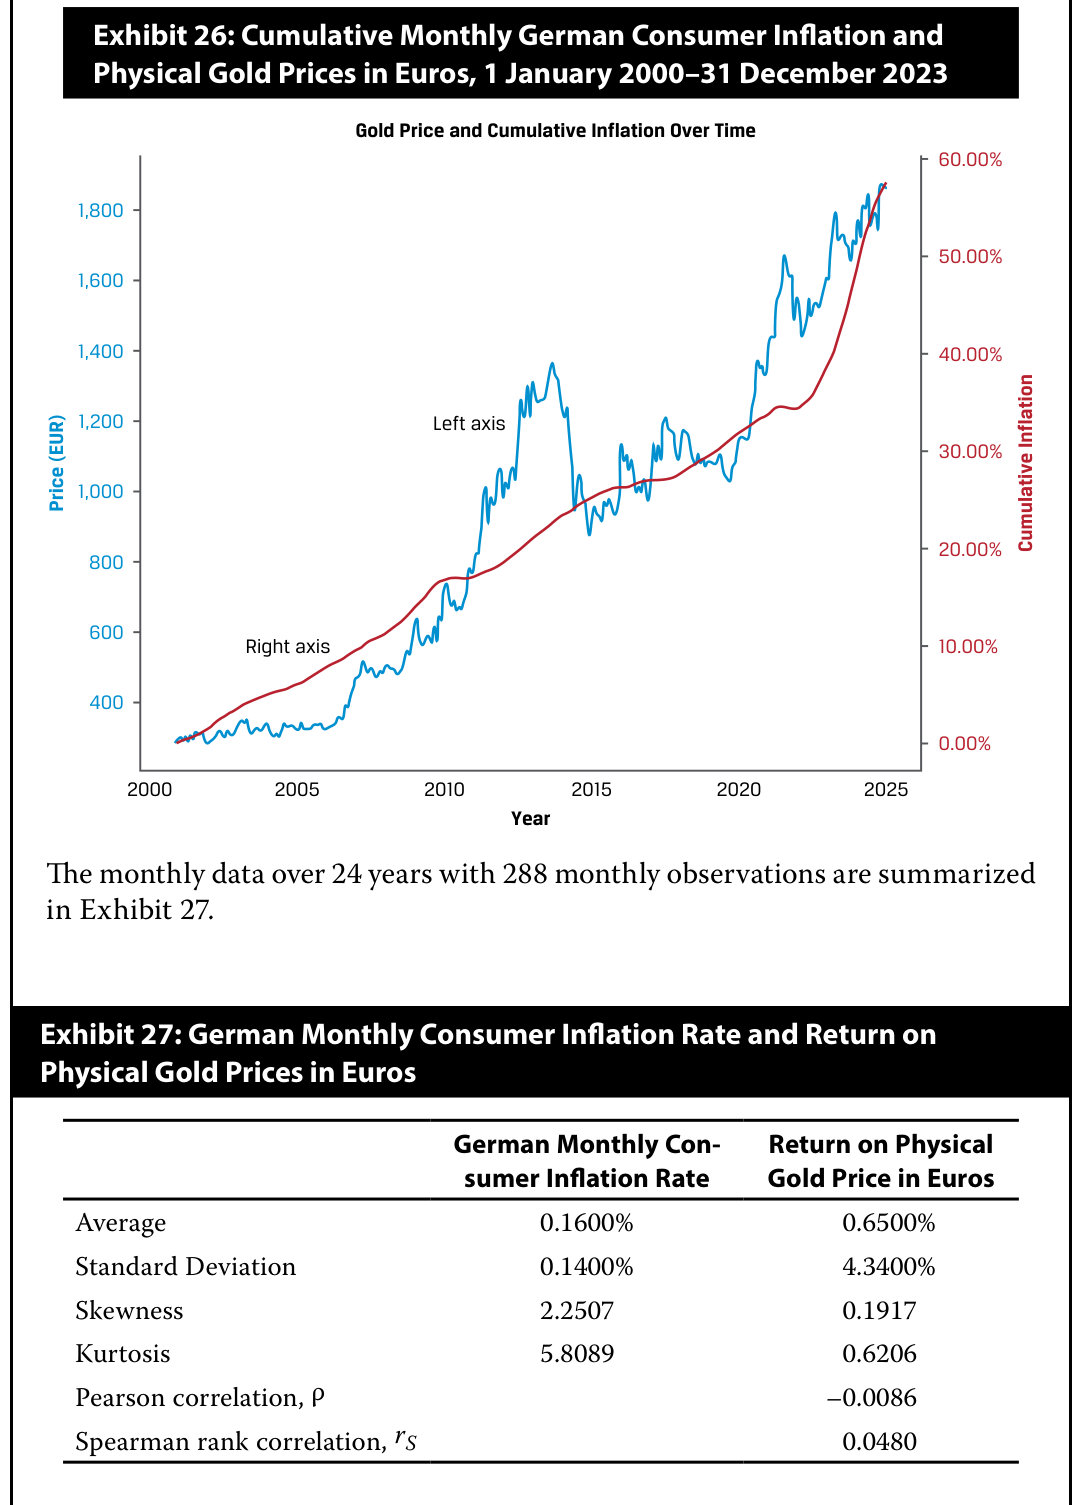
\includegraphics[width=0.75\linewidth]{002_figs/007_Module_7/exhibit_26.png}
	\caption{German Consumer Inflation and Physical Gold Prices (EUR)}
	\label{fig:mod7_exhibit_26}
\end{figure}
% Reference: CFA Curriculum 2027, Volume 1, Module 7, Page 371, Exhibit 26

\begin{figure}[!htbp]
	\centering
	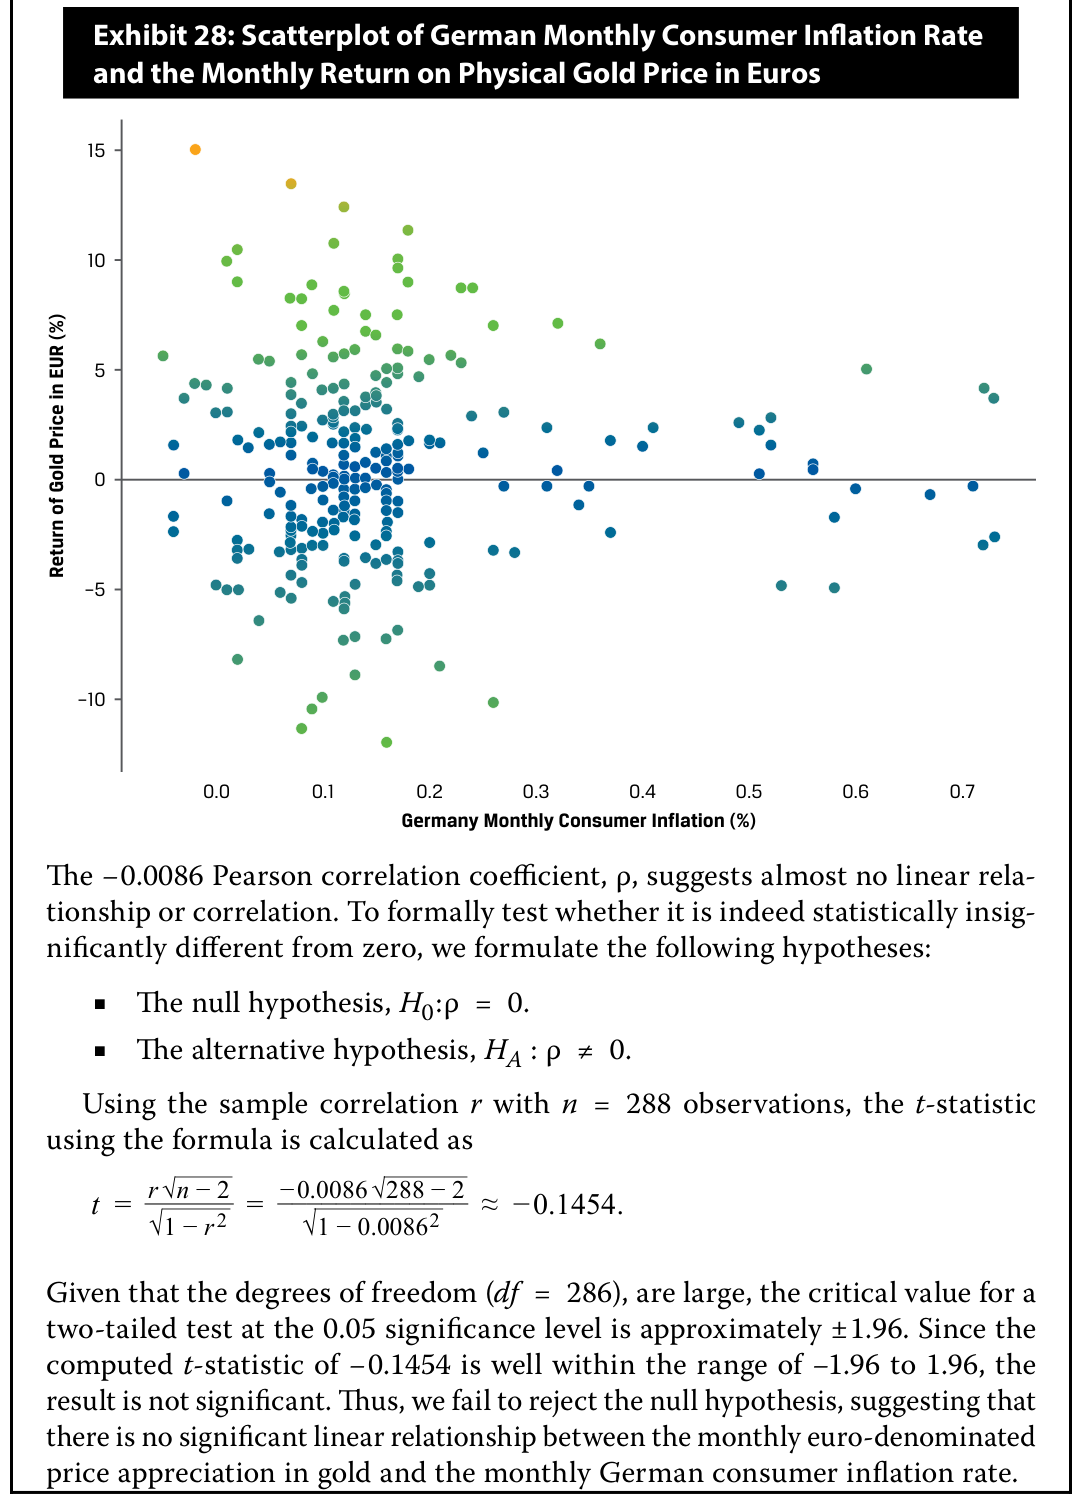
\includegraphics[width=0.75\linewidth]{002_figs/007_Module_7/exhibit_28.png}
	\caption{Scatterplot of German Inflation and Gold returns}
	\label{fig:mod7_exhibit_28}
\end{figure}
% Reference: CFA Curriculum 2027, Volume 1, Module 7, Page 372, Exhibit 28

\subsection{Chi-Square Test of Independence}
For categorical data, we test whether classifications are independent using a Chi-square test statistic with $df = (r - 1)(c - 1)$:
\begin{equation}
	\chi^2 = \sum_{i=1}^r \sum_{j=1}^c \frac{(O_{ij} - E_{ij})^2}{E_{ij}}
	\label{eq:chisq_independence_m7}
\end{equation}
% Reference: CFA Curriculum 2027, Volume 1, Module 7, Page 375, Equation (14)

Where $O_{ij}$ is the observed frequency and $E_{ij}$ is the expected frequency assuming independence:
\begin{equation}
	E_{ij} = \frac{(\text{Total Row } i) \times (\text{Total Column } j)}{\text{Overall Total } N}
	\label{eq:expected_freq_m7}
\end{equation}
% Reference: CFA Curriculum 2027, Volume 1, Module 7, Page 374, Equation (13)

Standardized residuals help identify which cells deviate significantly (values exceeding $\pm 1.96$ are significant):
\begin{equation}
	\text{Standardized Residual} = \frac{O_{ij} - E_{ij}}{\sqrt{E_{ij}}}
	\label{eq:standardized_residual_m7}
\end{equation}
% Reference: CFA Curriculum 2027, Volume 1, Module 7, Page 377, Equation (15)

\begin{tcolorbox}[
	colback=gray!5!white,
	colframe=black!15!white,
	boxrule=0.5pt,
	arc=3pt,
	title=\textbf{Case Study: Comparing Environmental and Governance Ratings},
	coltitle=black,
	colbacktitle=black!5!white,
	before skip=6pt,
	after skip=6pt,
	breakable
]
We examine the independence of ESG ratings of 500 firms (Table~\ref{tab:esg_contingency_m7}). Expected frequency $E_{22}$ (Average/Average) is $\frac{260 \times 230}{500} = 119.6$. Summing scaled squared deviations (Exhibit~\ref{fig:mod7_exhibit_31}), we obtain $\chi^2 \approx 35.75$. With $df = (3-1)(3-1) = 4$, the critical value at 5\% is $\chi^2_{0.05} = 9.49$. Since $35.75 > 9.49$, we reject the null hypothesis of independence. Environmental and governance ratings are related.
\end{tcolorbox}

\begin{table}[!htbp]
\centering
\caption{ESG Ratings Contingency Table ($N=500$)}
\label{tab:esg_contingency_m7}
\begin{tabular}{p{0.35\linewidth} p{0.15\linewidth} p{0.13\linewidth} p{0.12\linewidth} p{0.10\linewidth}}
\toprule
\textbf{Environmental Rating} & \textbf{Progressive (GR1)} & \textbf{Average (GR2)} & \textbf{Poor (GR3)} & \textbf{Total} \\
\midrule
\textbf{Progressive (ER1)} & 35 & 40 & 5 & 80 \\
\textbf{Average (ER2)} & 80 & 130 & 50 & 260 \\
\textbf{Poor (ER3)} & 40 & 60 & 60 & 160 \\
\midrule
\textbf{Total} & 155 & 230 & 115 & 500 \\
\bottomrule
\end{tabular}
\end{table}
% Reference: CFA Curriculum 2027, Volume 1, Module 7, Page 373, Exhibit 29

\begin{figure}[!htbp]
	\centering
	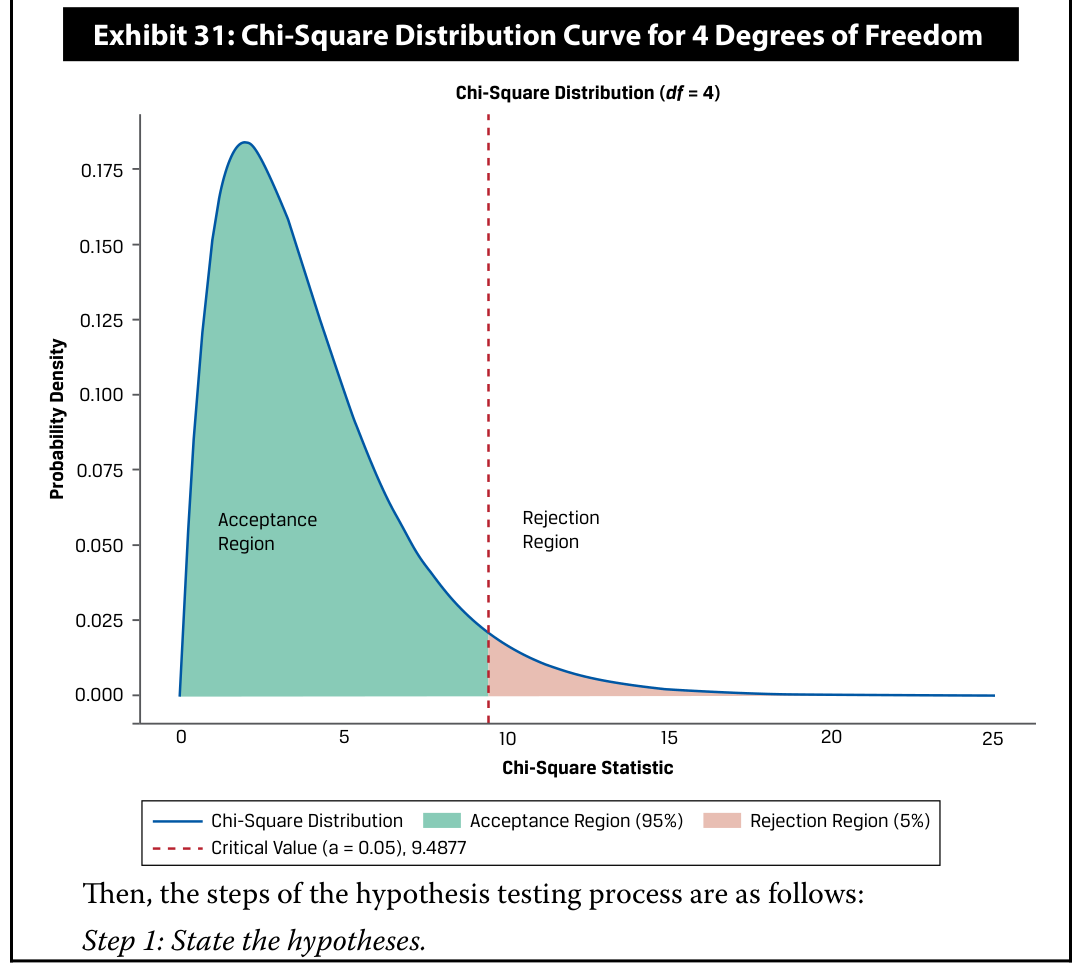
\includegraphics[width=0.75\linewidth]{002_figs/007_Module_7/exhibit_31.png}
	\caption{Chi-Square Distribution Curve with 4 Degrees of Freedom}
	\label{fig:mod7_exhibit_31}
\end{figure}
% Reference: CFA Curriculum 2027, Volume 1, Module 7, Page 375, Exhibit 31

\begin{tcolorbox}[
	colback=gray!5!white,
	colframe=black!15!white,
	boxrule=0.5pt,
	arc=3pt,
	title=\textbf{Case Study: Fund Size and Investment Style of 1,594 ETFs},
	coltitle=black,
	colbacktitle=black!5!white,
	before skip=6pt,
	after skip=6pt,
	breakable
]
We test whether ETF size and investment style are independent (Table~\ref{tab:etf_contingency_m7}). Calculated expected frequencies and scaled squared deviations yield $\chi^2 = 32.07$ (Exhibit~\ref{fig:mod7_exhibit_35}). With $df = 4$, the critical value at 1\% is $13.28$. Since $32.07 > 13.28$, we reject the null hypothesis of independence. 
Analyzing standardized residuals (Exhibit~\ref{fig:mod7_exhibit_36}), the cell for Medium-Growth has a residual of $+3.69$ (significantly higher than expected), and Large-Growth has a residual of $-2.72$ (significantly lower than expected).
\end{tcolorbox}

\begin{table}[!htbp]
\centering
\caption{ETFs Classifications Contingency Table ($N=1,594$)}
\label{tab:etf_contingency_m7}
\begin{tabular}{p{0.25\linewidth} p{0.15\linewidth} p{0.15\linewidth} p{0.15\linewidth} p{0.15\linewidth}}
\toprule
\textbf{Investment Type} & \textbf{Small} & \textbf{Medium} & \textbf{Large} & \textbf{Total} \\
\midrule
\textbf{Value} & 50 & 110 & 343 & 503 \\
\textbf{Growth} & 42 & 122 & 202 & 366 \\
\textbf{Blend} & 56 & 149 & 520 & 725 \\
\midrule
\textbf{Total} & 148 & 381 & 1,065 & 1,594 \\
\bottomrule
\end{tabular}
\end{table}
% Reference: CFA Curriculum 2027, Volume 1, Module 7, Page 377, Exhibit 33

\begin{figure}[!htbp]
	\centering
	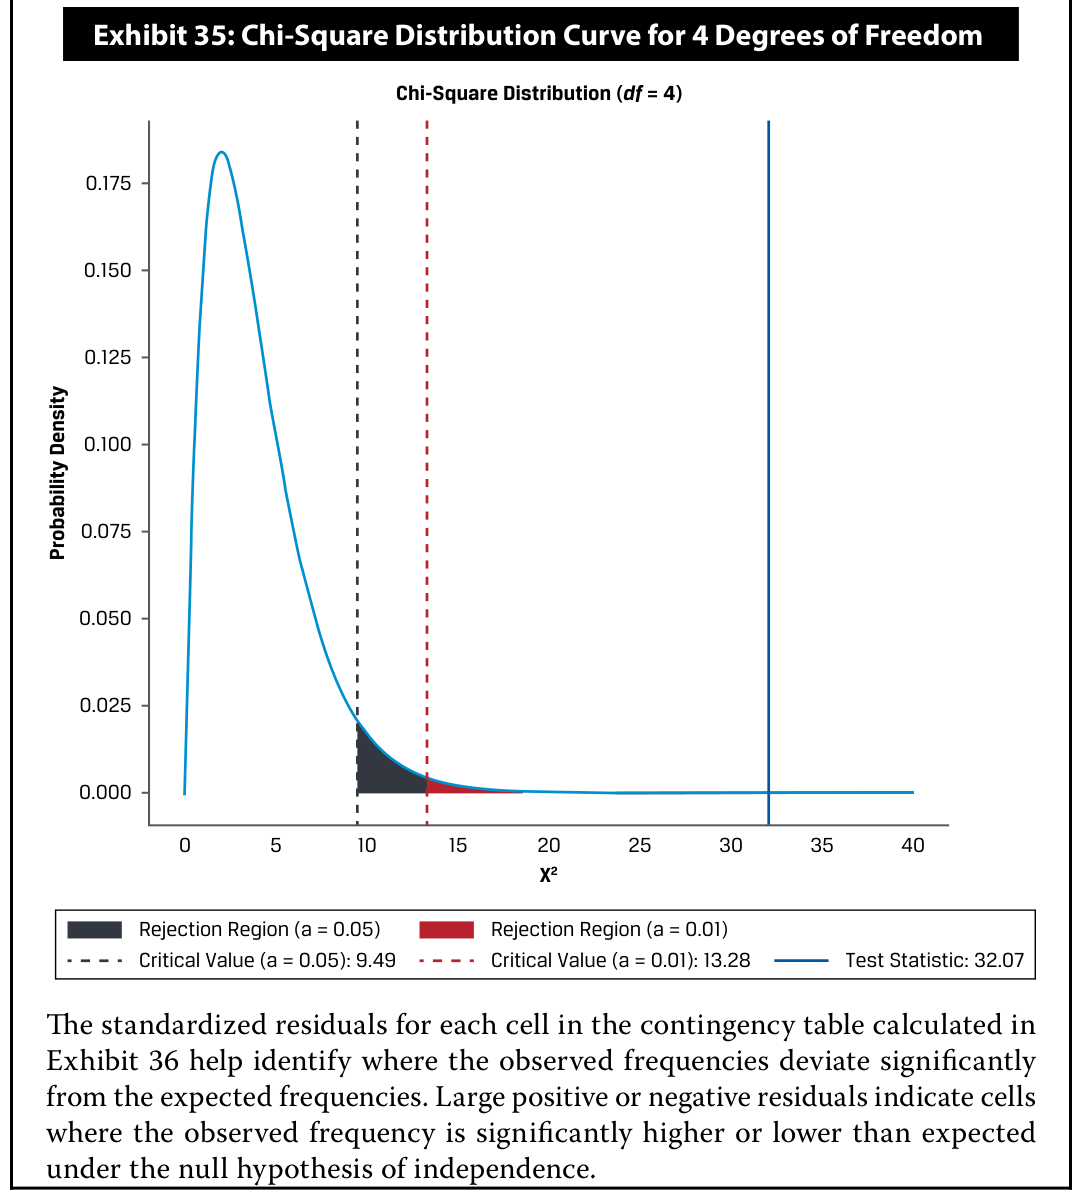
\includegraphics[width=0.75\linewidth]{002_figs/007_Module_7/exhibit_35.png}
	\caption{Chi-Square Rejection Regions for ETF Independence Test ($df=4$)}
	\label{fig:mod7_exhibit_35}
\end{figure}
% Reference: CFA Curriculum 2027, Volume 1, Module 7, Page 379, Exhibit 35

\begin{figure}[!htbp]
	\centering
	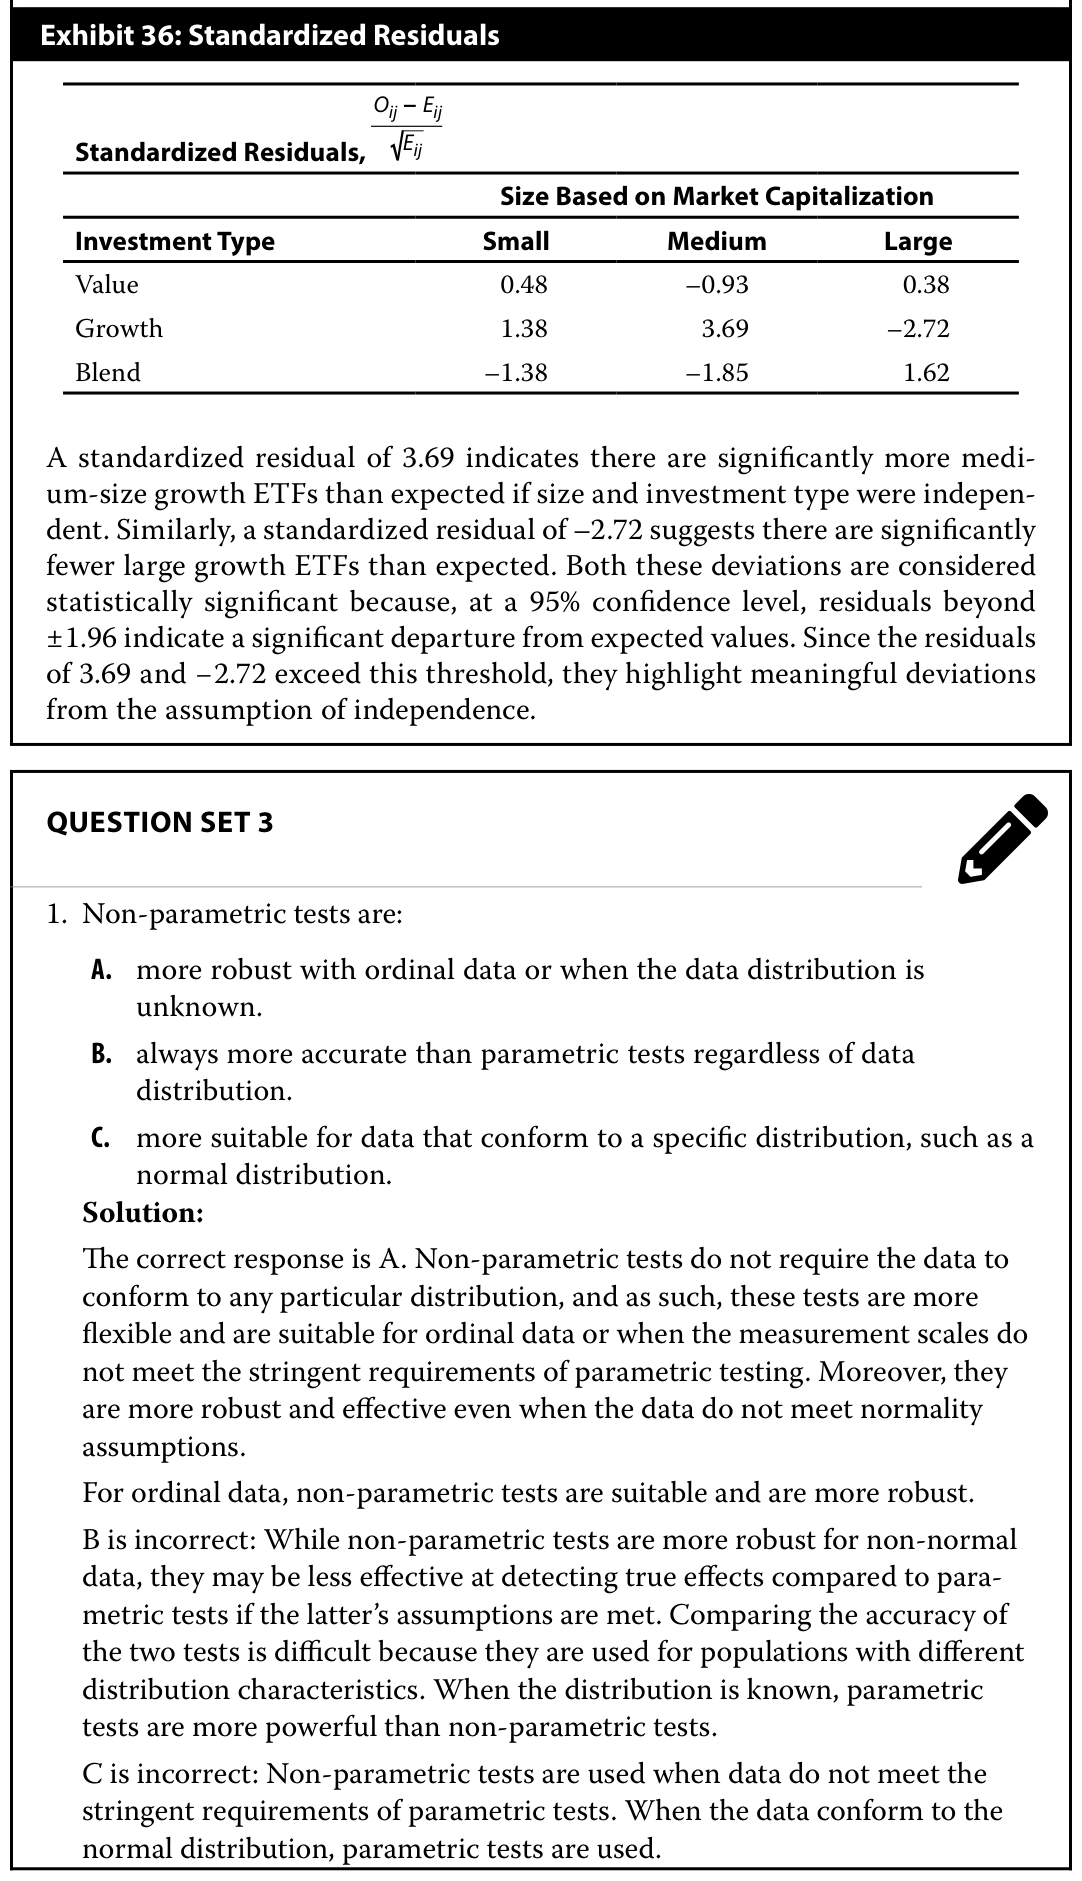
\includegraphics[width=0.75\linewidth]{002_figs/007_Module_7/exhibit_36.png}
	\caption{Standardized Residuals plot for Size vs Style of ETFs}
	\label{fig:mod7_exhibit_36}
\end{figure}
% Reference: CFA Curriculum 2027, Volume 1, Module 7, Page 380, Exhibit 36
